\section{Basic Concepts}
\label{section:basicConcepts}
% Darstellung des aktuellen Wissens zum Thema (Literaturphase – Grundlagen)
% Hier ist ein Überblick über das Fachthema und die Begrifflichkeiten sowie eine Darstellung bestehender Lösungsansätze/Technologien anhand von Quellen aus der wissenschaftlich-technischen Literatur zu erarbeiten. Besonderes Augenmerk ist auf die korrekte Zitierweise von Quellen zu legen. Anderen LeserInnen der Arbeit soll damit das Verständnis für die darauf folgenden Teile der Arbeit erschlossen werden. Inhalte flüchtiger Quellen (Websites) sind geeignet, müssen aber gesichert werden (CD/DVD).

% zusammenfassung aller themen einfügen 
In this chapter, the existing web platform Easydrum and its technologies gets introduced, as well as the concepts of a drum set and its notation. Subsequently, an overview to audio signal processing, onset detection, different methods for classification and the Web Audio API is given. Thereby, the features and technologies required for the methods developed in this thesis can get pointed out which.

\subsection{Easydrum} \label{section:Easydrum}

\begin{figure}[ht]
	\centering
	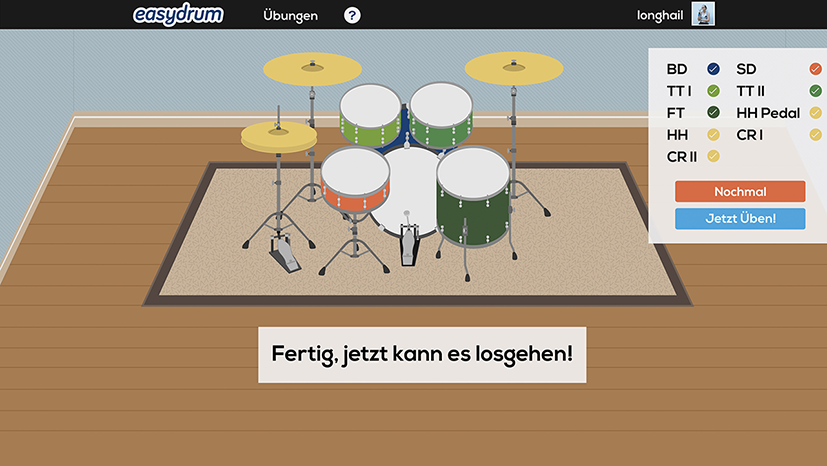
\includegraphics[width=\textwidth]{images/Easydrum/configuratorscreen.png}
	\caption{Easydrum drum configurator.}
	\label{fig:configuratorscreen}
\end{figure}

Easydrum is a free e-learning platform on the web. It provides a couple of different exercises for learning how to play a drum set. The user gets an introduction to the different components of the drum set and learns to read drum sheets. What makes the platform unique is the possibility to connect an e-drum set to it via USB to play the exercises. After connecting, the MIDI signals produced by the e-drum set can be read and processed by the platform. This way, giving feedback to the user during playing an exercise is facilitated. Before the e-drums can be used for exercising, they have to be configured with the provided e-drum configurator. Here, the user has to play each drum once to save the appropriate MIDI signal. In addition to an e-drum set, the computer keyboard can be used for exercising as well.

The application displays the exercises as drum sheets. When the exercise started, the notes are moving over the sheet. A highlighted hit area on the sheet shows the point in time when a note needs to be played. Further on, an illustration of a drum set animates the exercise while playing it. By using a configured e-drum set or the computer keyboard, the application can recognize if the right drums are stroked at the right time. The played notes are added to the sheets in real-time to show the user if he hit or missed a note. After the exercise is finished, the user gets rewarded with zero to 100 points and zero to three stars, depending on the hit-rate.

\begin{figure}[ht]
	\centering
	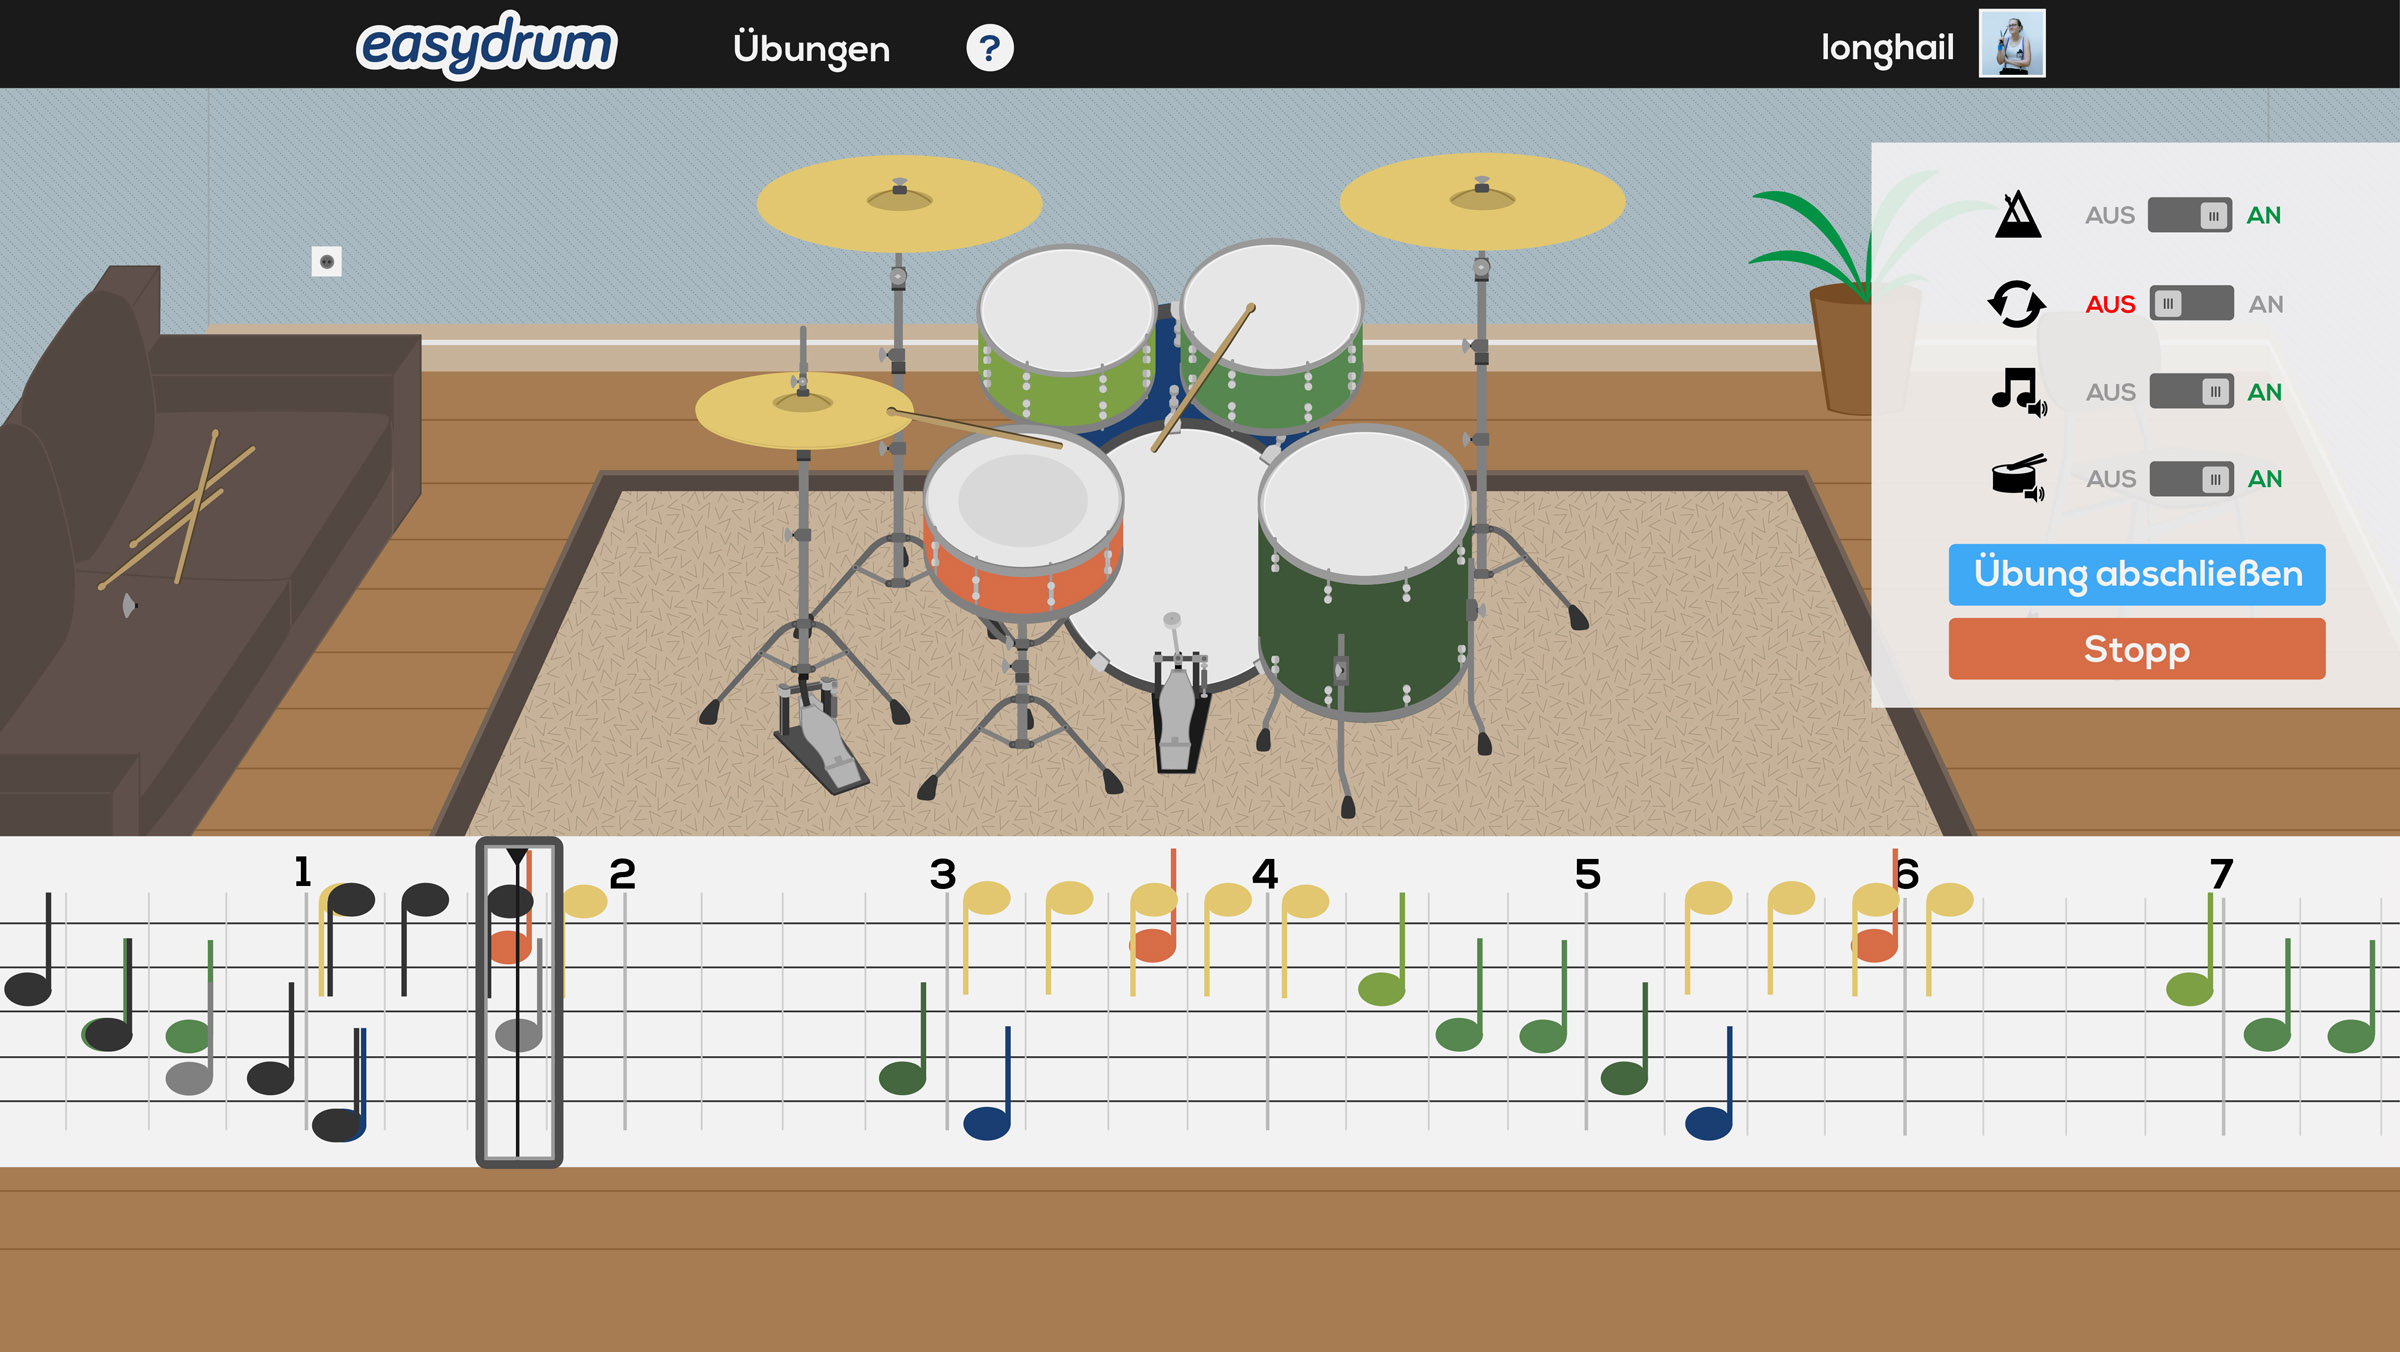
\includegraphics[width=\textwidth]{images/Easydrum/exerciseplayerscreen.png}
	\caption{Easydrum exercise player.}
	\label{fig:exerciseplayerscreen}
\end{figure}

The application is build on the open-source web framework Ruby on Rails. An overview to the framework is given on their web site \autocite{RubyOnRails:2015}. For this thesis two components of the web site are important for a detailed analysis. The e-drum configurator on the one hand and the exercise player on the other hand. Screenshots of the existing drum configurator and exercise player are shown in figures \ref{fig:configuratorscreen} and \ref{fig:exerciseplayerscreen}. 


\newpage
\newpage

\subsubsection{Technologies}
The components of Easydrum largely run in the web frontend with the help of JavaScript. 

JavaScript is a scripting language published in 1995 to supplement HTML and thus enable easy interactions with the Netscape Navigator browser. The language developed quickly from an easy scripting language to a widely used standard in web applications. It has been documented under the ECMAScript standard by the Ecma International organization. Today, JavaScript runs in all major browsers and thus enables the development of modern interactive web applications, which can run on the web frontend with high performance. Current browsers support ECMAScript 5, whereas a sixth version already exists and will be adopted to browsers, in the future. A detailed introduction to JavaScript can be found in \autocite{Haverbeke:2014}.

In addition to JavaScript, Easydrum uses jQuery and the jQuery UI widget factory. According to the jQuery web site \autocite{jQuery:2015}, jQuery is `a fast, small, and feature-rich JavaScript library. It makes things like HTML document traversal and manipulation, event handling, animation, and Ajax much simpler with an easy-to-use API that works across a multitude of browsers'. The jQuery UI widget factory provides a framework that enables developers to write stateful jQuery plug-ins, so-called widgets. It provides object oriented methods to manage the life cycle of a widget, which includes creating and destroying a widget, changing options, making super calls and receive event notifications. The jQuery UI widget factory is documented in \autocite{jQueryUI:2015}.

The key feature in the existing application is the method for receiving MIDI events from the connected e-drum set. Therefore, Easydrum uses the Web MIDI API, which is supporting the MIDI protocol. It enables web applications to communicate with MIDI input and output devices. The Web MIDI API specification was published by the W3C Audio Working Group as a Working Draft \autocite{WebMidiApi:2015}. Thus, it is not yet an official web standard and it is also not yet implemented in all common browsers but is intended to become a standard. The actual Easydrum application is able to run without an additional plug-in in Google Chrome. For other browsers the Jazz-Plugin \autocite{JazzPlugin:2015} has to be installed to receive MIDI input. As soon as the Web MIDI API is accessible via the other browsers, the plug-in will no longer be needed. 

\subsubsection{Architecture}

The basic architecture of the Easydrum application is show in figure \ref{fig:Easydrumarchitecture}. As mentioned before, the player largely runs in the web frontend with the help of JavaScript and the jQuery UI widget factory. 

\begin{figure}[ht]
	\centering
	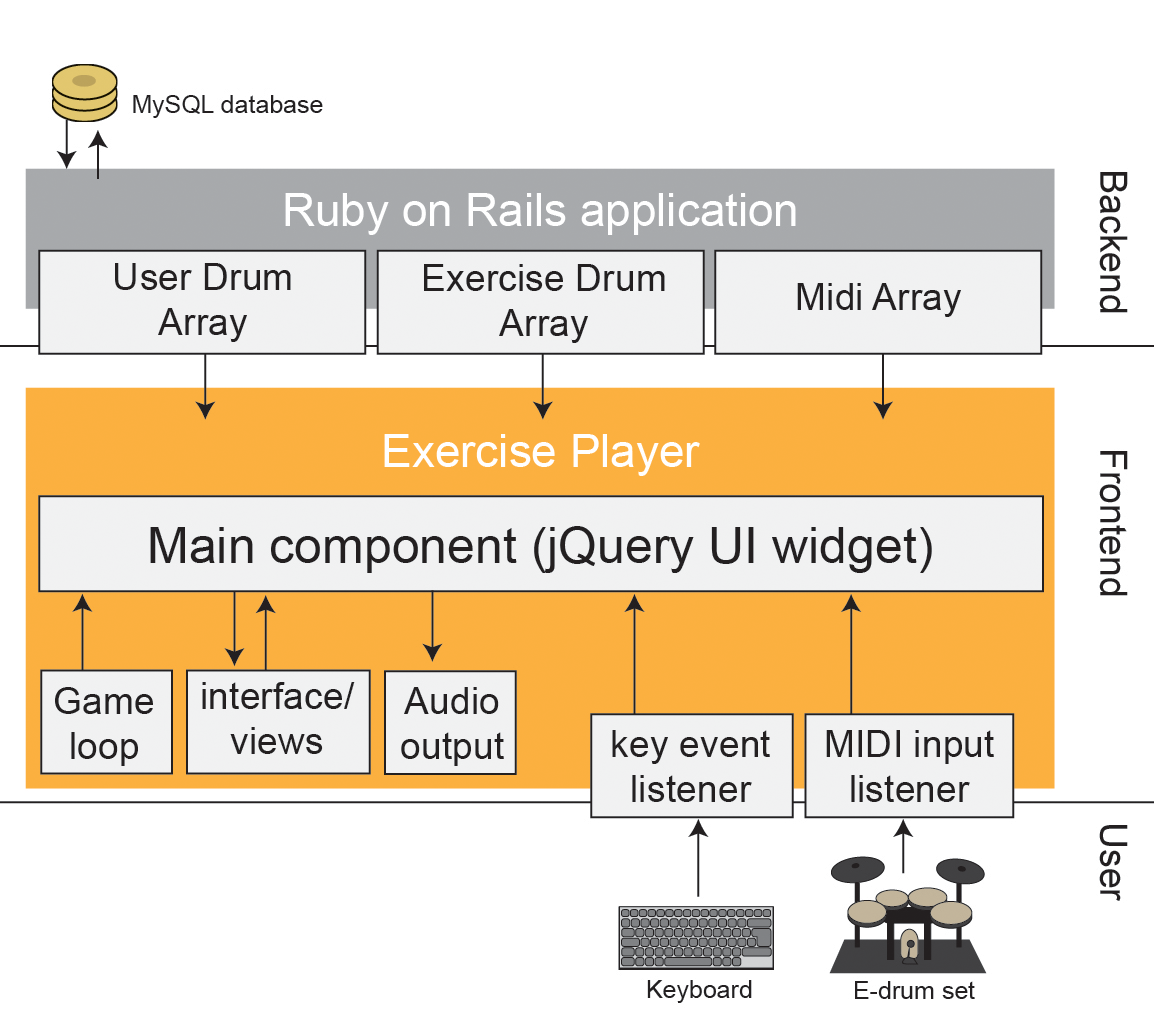
\includegraphics[width=.8\textwidth]{images/Easydrum/app_architcture.png}
	\caption{Easydrum application architecture.}
	\label{fig:Easydrumarchitecture}
\end{figure}

One main jQuery UI widget connects all components of the player. These components are the game loop, the views, two input listeners and the audio output. Each event in one of these components is sent to the main widget. The main widget processes all events and subsequently updates the relevant components. If an exercise is playing, the game loop adjusts the number of frames per seconds depending on the calculation power of the used computer. It invokes an event called \textit{tick} for every frame.

The main widget needs three arrays to be initialized. The first two arrays contain data for an e-drum set. They define the MIDI data mapped to appropriate drums. One of the drum arrays contains the data for the e-drum set used to record the exercise, the other contains the data for the drum set of the actual user. The third array contains the MIDI data that describe the actual exercise.

The input data is received by the two listeners. There is one listener that is able to receive MIDI data and one that is able to receive key events from the computer keyboard. These listeners are initialized with the user drum array described in the preceding. With the help of this array the input is mapped to the played drum and note. For every played drum the note value and the point in time when it was played is saved.

Hence, to extend the application to work with an acoustic drum set, a new listener, which maps audio input to played drums, needs to be developed and appended to the main widget.

\subsection{Components of a Drum Set}

The developed Easydrum extension receives audio data from an analog drum set. To understand these methods, the instrument and its components are introduced below.

\begin{figure}[htb]
	\centering
	\subfloat[1 - hi-hat, 2 - snare drum, 3 - bass drum 4 - tom 1, 5 - tom 2, 6 - tom 3,  7 - crash cymbal, 8 - ride cymbal]{
		\includegraphics[height=6.0cm]{images/drumset/drumset_02.jpg}
		\label{fig:components}
	}
	\qquad
	\subfloat[Rim, bow and bell of a cymbal.]{
		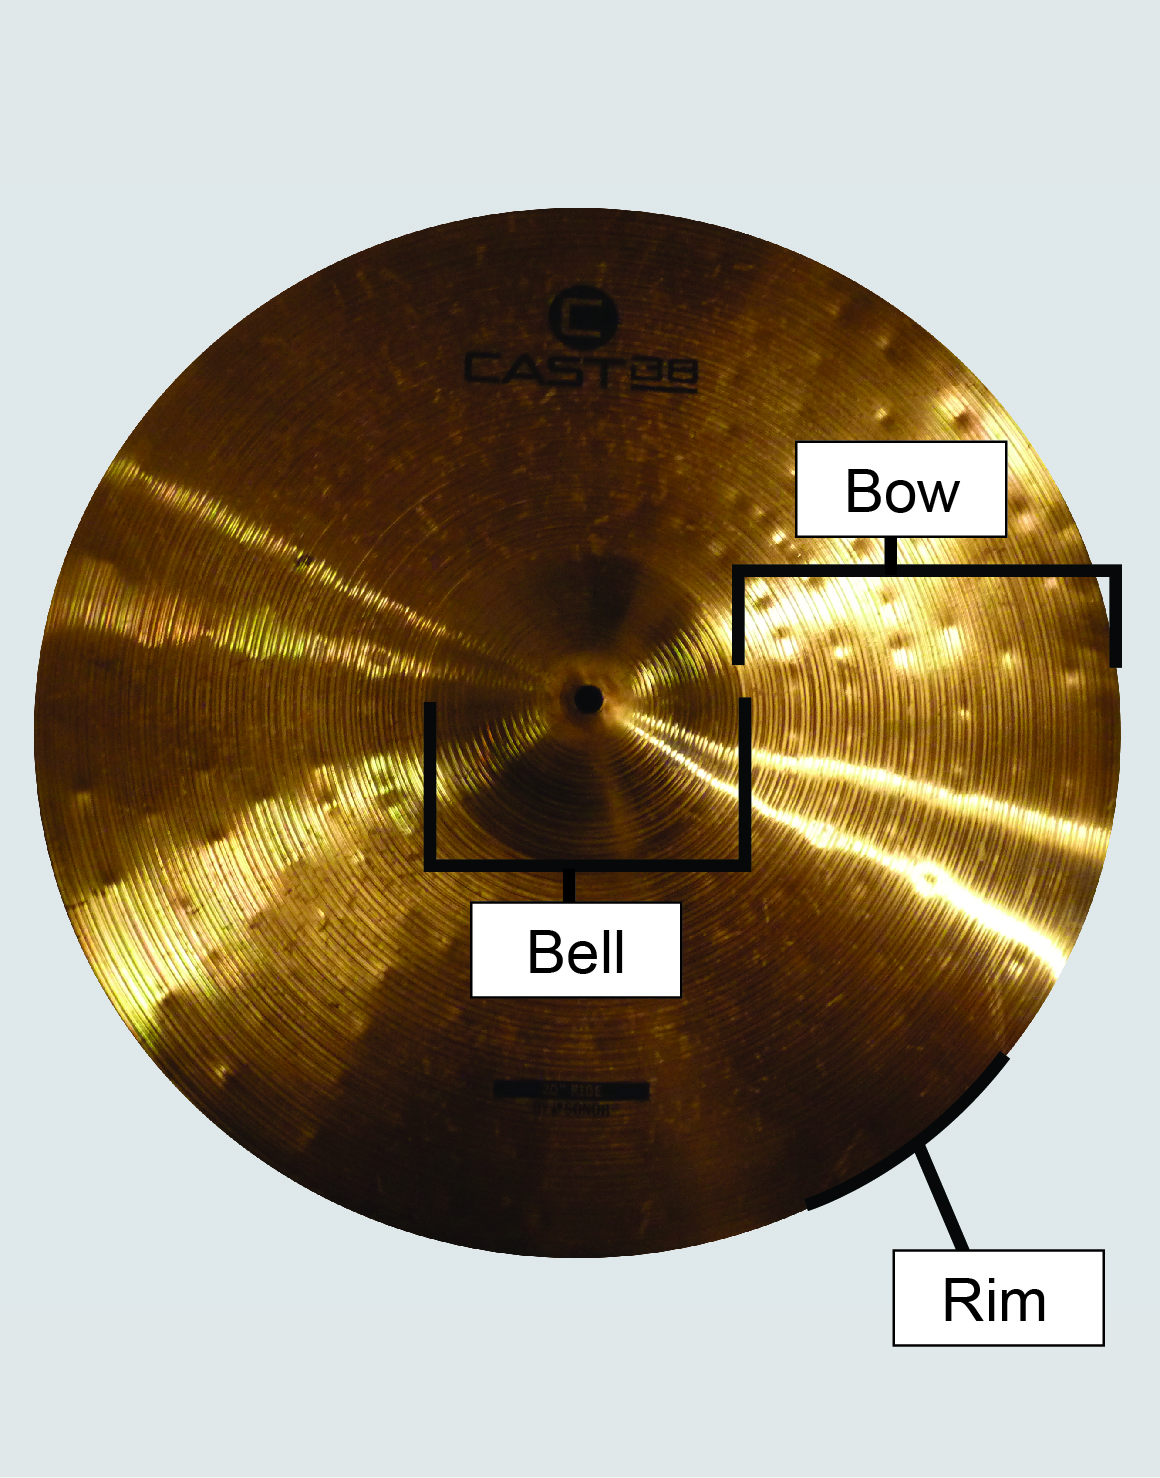
\includegraphics[height=6.0cm]{images/drumset/ride.jpg}
		%for reference of this subfigure only
		\label{fig:rim_bow_bell}
	}
	\caption{
		Components of a standard drum set.
	}
	\label{fig:drumset}
\end{figure}

A drum set is a percussive instrument. Percussive instruments are one of the oldest types of instruments in history. Today, a wide range of different instruments of this type have been created. Thus, a drum set can consist of various numbers of different drums, cymbals and other components, such as woodblocks, bells and triangles. To limit the possibilities, this thesis merely uses a standard drum set.

A standard drum set, as displayed in figure \ref{fig:components}, consists of eight different drums, which are a bass drum, a snare drum, two rack toms, a floor tom, a hi-hat, a ride cymbal and a crash cymbal. The bass drum is the central element of the drum set. Strokes are made with the help of a foot pedal. Together with the hi-hat and the snare drum, the bass drum defines the rhythm of a piece of music. The hi-hat consists of two cymbals that can be closed by a foot pedal. Thus, it can be played either opened or closed. The toms and cymbals are primarily used to play fill-ins\footnote{musical phrases between melody or song segments} and accents. As shown in figure \ref{fig:rim_bow_bell}, the cymbals consist of three components which create different sounds. These are the rim, the bow and the bell, whereas the rim is the utter part of the cymbal, the bell is a bulge in the center of it and the bow is the area on the top between the rim and the bell.


\subsection{Notation}

Typically, sheets are used to visualize a drum rhythm. Thus, in this thesis, drum sheets are used to visualize the tested drum rhythms in section \ref{section:onsetdetectionmethod}. To understand these sheets, the drum notation is explained in the following.

A sheet contains different elements like staff, clef, notes, pauses and bars, which are used to build a rhythm. A sample sheet is shown in figure \ref{fig:sheetExample}.

\begin{figure}[h]
	\centering
	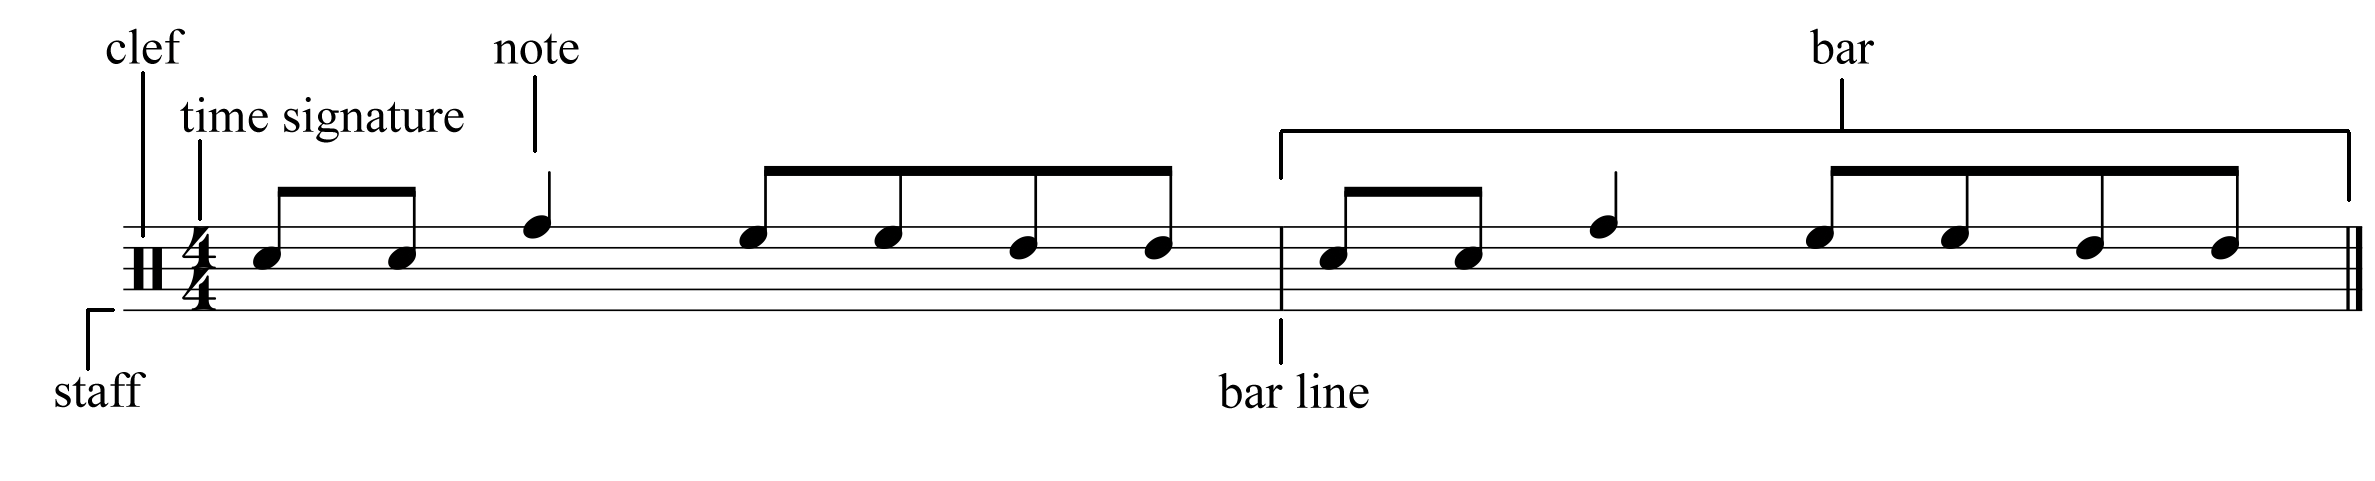
\includegraphics[width=\textwidth]{images/drumsandsheets/example.png}
	\caption{Example drum sheet.}
	\label{fig:sheetExample}
\end{figure}

The staffs are the horizontal lines on which the notes are placed. A sheet contains five staffs. 

The meaning of the particular notes is defined by the used clef. The clef is placed at the beginning of each sheet. Common clefs are for example the treble clef or the bass clef. A neutral clef is used for drum sets. In contrast to the notation of most clefs, the position of a note on the staff does not indicate its pitch, but symbolizes the component of the used drum kit that has to be stroked. Thereby, different notations are used for drum sets. Hence, to explain which note symbolizes which drum, a so called 'drum key' is used. Generally, round note heads are used for drums and x-shaped ones for cymbals. If a stroke is performed by a stick, the stem of the appropriate note is placed from the note head upwards and if it is performed with a foot pedal from the note head downwards. For this thesis, the drum key shown in figure \ref{fig:sheetNotation} is used.

\begin{figure}[h]
	\centering
	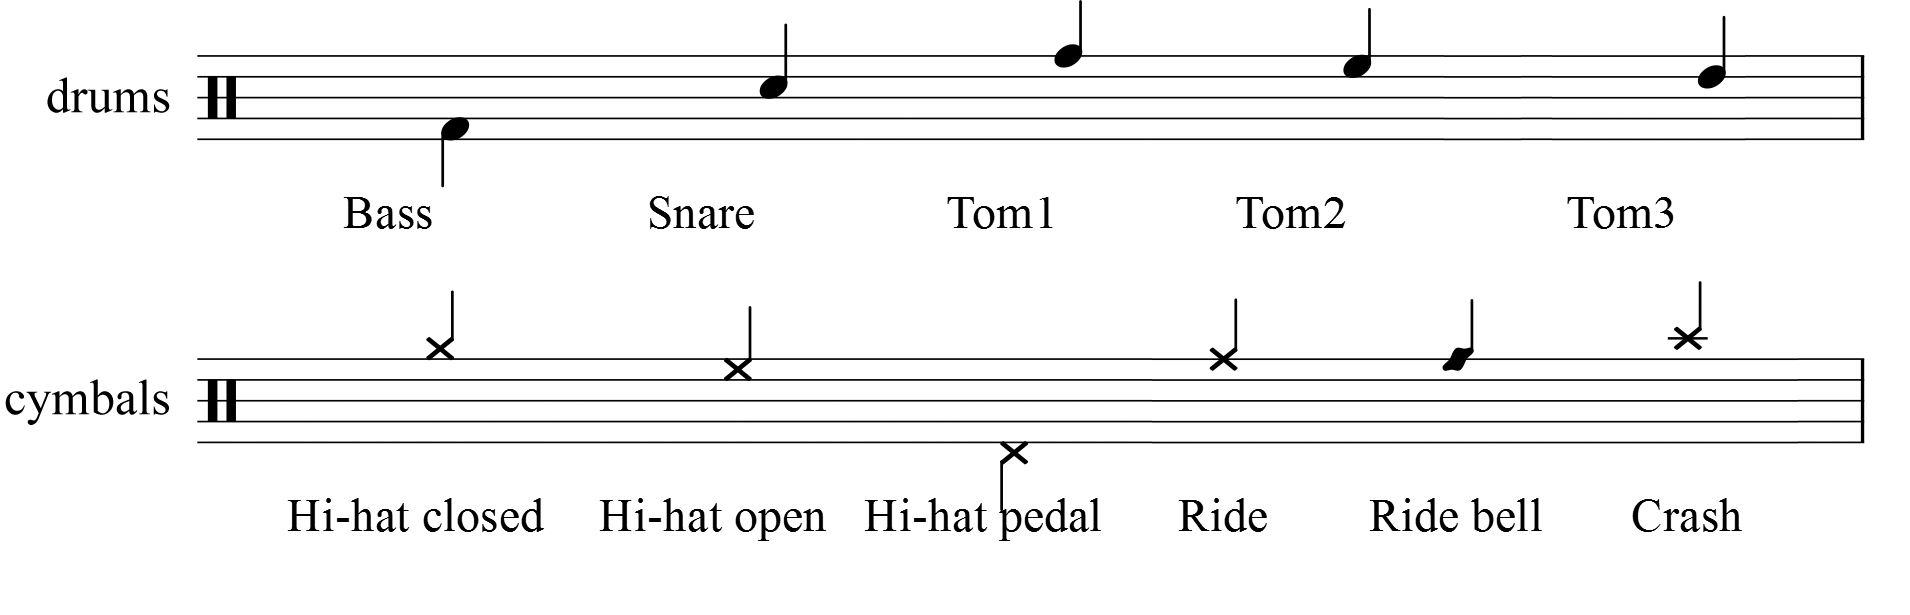
\includegraphics[width=\textwidth]{images/drumsandsheets/notation.png}
	\caption{Drum notation.}
	\label{fig:sheetNotation}
\end{figure}

The notes on the sheet are segmented in small blocks called bars. The bars are separated on the sheet by bar lines.

The number and type of beats in a bar is predefined by the time signature. The time signature is given in the beginning of the sheet after the clef. Example time signatures are $\frac44$, $\frac34$ or $\frac48$. The upper number specifies the number of beats in which the bar is separated and the lower one specifies the note value of a single beat. The note value defines the duration of a note. For this thesis, only the time signature $\frac44$ is used. For this time signature there are counted four beats in one bar, which have the value of a quarter note. 

Important note values in this thesis are the whole note, the halve note, the quarter note, the eighth note and the sixteenth note. The whole note has the length of four quarters and thus has the duration of a whole bar with the time signature $\frac44$. The duration of the recent notes is given proportional to the quarter note. By putting a dot behind a note, the note duration is stretched by the next lower note value. Next to notes, pauses can be displayed. Pauses specify a certain period of time, where no note is played. They can have the same values as notes. Different note and pause values are shown in figure \ref{fig:sheetValues}.

\begin{figure}[h]
	\centering
	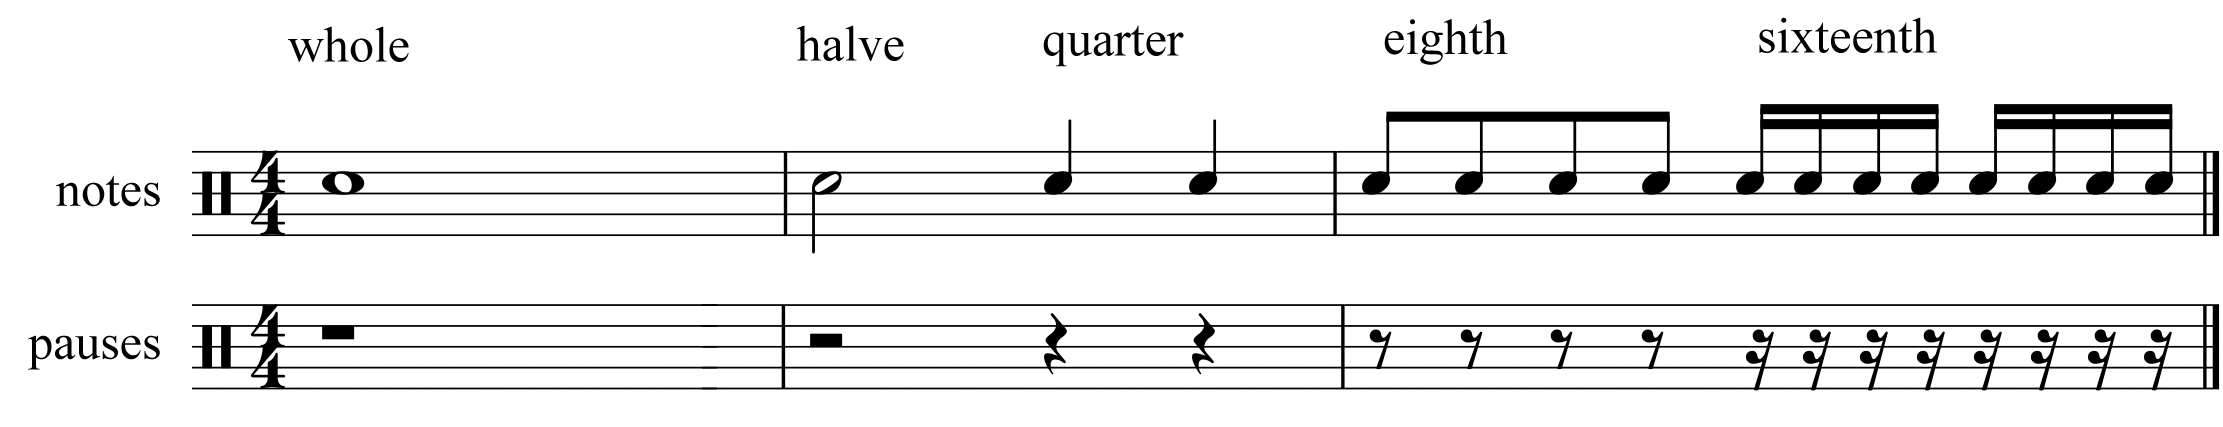
\includegraphics[width=\textwidth]{images/drumsandsheets/note_values.png}
	\caption{Note and pause values.}
	\label{fig:sheetValues}
\end{figure}

In addition to the time signature, the beats per minute (bpm) of a rhythm can be specified . For instance, if a beat is played with 60 bpm, this means one beat per second is played.

More information about the drum notation can be found in \autocite{Stein:2013}.

\subsection{Audio Signal Processing}

Every stroke on a drum or a cymbal creates an analog acoustic signal. This signal is a sinusoidal signal that contains information about the character of the sound it produces. To receive and process this information on a computer, the sounds need to be converted into digital signals. The steps of this process are called sampling and quantization. To provide an insight into the structure of audio signals and the process of quantization, these subjects are introduced in the following. An introduction to signal processing is also given in \autocite{Werner:2012}.

\subsubsection{Audio Signals}

An analog audio signal is a value- and time-continuous, sinusoidal wave. A sample audio signal is shown in figure \ref{fig:audiosignal}. The wave is build by the time $t$ in seconds as x-axis and the amplitude $y(t)$ as y-axis.

% figure audiosignal
\begin{figure}[h]
	\centering
	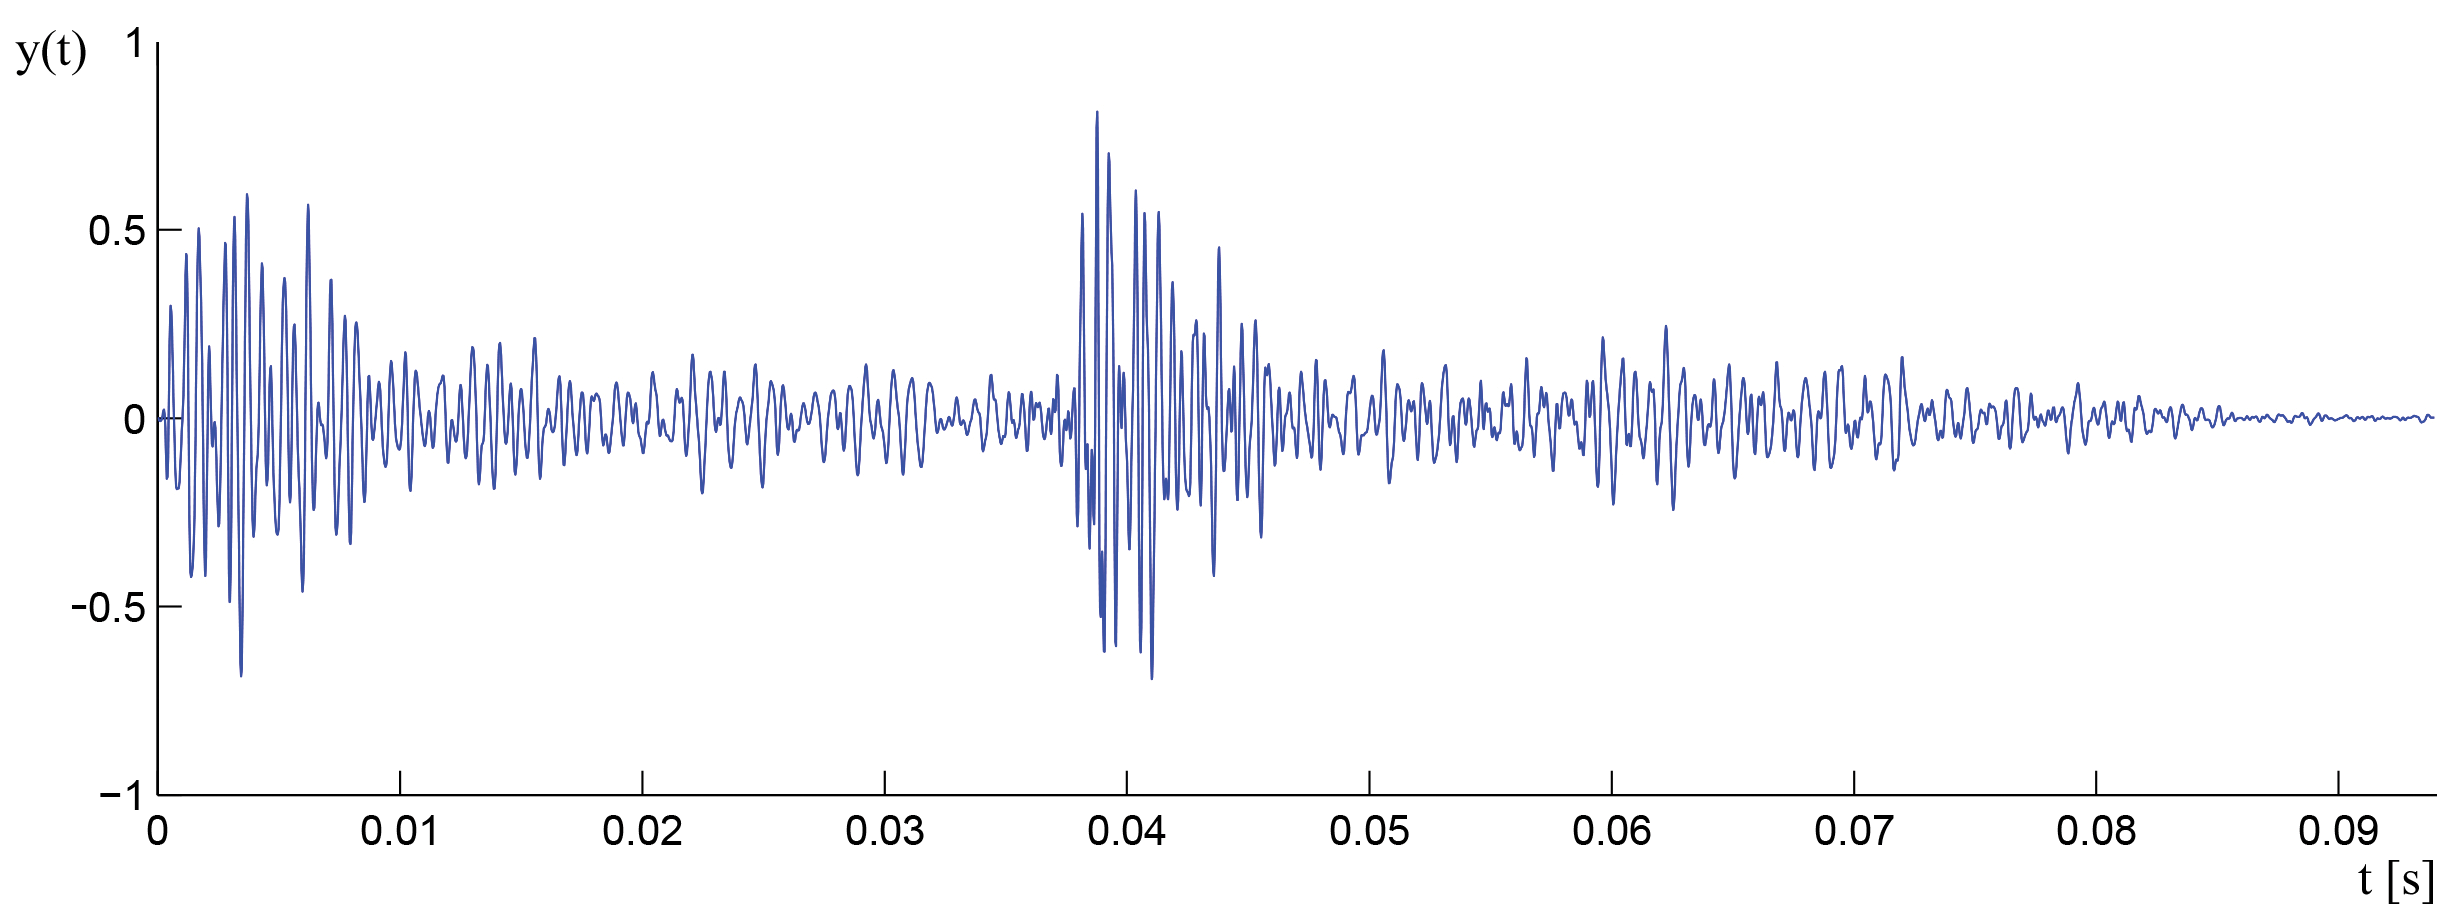
\includegraphics[width=.9\textwidth]{images/audiosignal.png}
	\caption{Example audio signal.}
	\label{fig:audiosignal}
\end{figure}

As introduced in \autocite{Weltner:2013}, the form of a periodic sinusoidal wave is described by its amplitude $A$, its period $\omega$ and its phase $\varphi_0$, as follows:
 
\begin{equation}
	y(t)=A*sin(\omega t+\varphi_0)
\end{equation}

An example sinusoidal wave is shown in figure \ref{fig:sinusoidalexample}. It shows the function
$y(t)=5*sin(2t+\frac{\pi}{2})$.

The amplitude $A$ defines the scaling factor for the sinus function. The maximum value of the function is always the value of this scaling factor. Thus, for $A=5$, the sinusoidal function has the maximum amplitude of $5$ and a minimum amplitude of $-5$.

The period $\omega$ defines the stretching and shrinking factor of the wave. For $\omega =1$, the sinusoidal function has a length of $2\pi$. For all values with $\omega <1$ the wave is stretched and for all values with $\omega >1$ it is shrunken.

The phase $\varphi_0$ defines the shifting of the wave on the x-axis. It is shifted to the left by positive values and to the right by negative values for $\varphi_0$. Considered within the unit circle, $\varphi_0$ describes a temporary shift of the wave by the phase angle $\varphi_0$. Figure \ref{fig:sinewave} shows a sinus function in relation to the phase angle in the unit circle.

%figure 1) function, einheitskreis
\begin{figure}[ht]
	\centering
	\subfloat[Sinus curve in relation to the unit circle.]{
		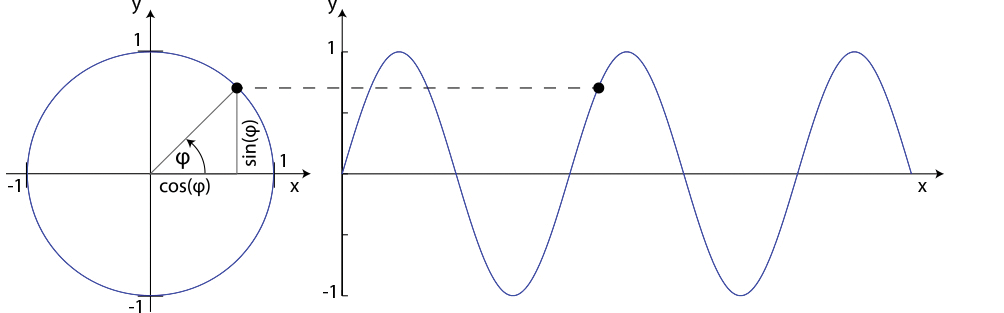
\includegraphics[height=3.0cm]{images/sine1.png}
		\label{fig:sinewave}
	}
	\subfloat[
	Example sinusoidal wave with 
	$y(t)=5*sin(2t+\frac{\pi}{2})$.
	]{
		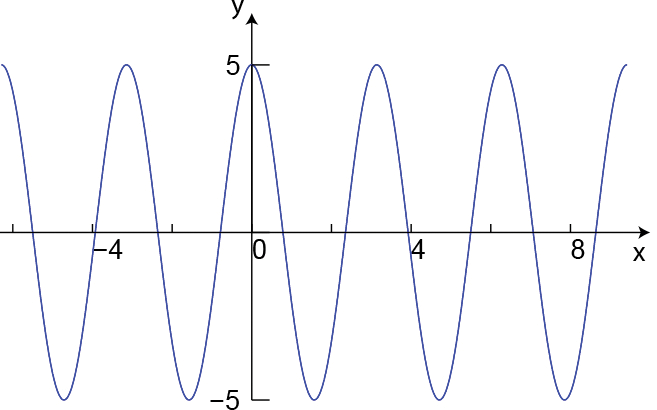
\includegraphics[height=3.0cm]{images/sine2.png}
		\label{fig:sinusoidalexample}
	}
	\caption{
		Sinusoidal functions.
	}
\end{figure}

As shown in figure \ref{fig:audiosignal}, an audio wave generally changes its form over time. Thus, it is an aperiodic signal, which can vary over time in its amplitude $A$, its period $\omega$ and its phase $\varphi_0$.

\subsubsection{Sampling and Quantization}

To process an audio signal on a computer, it needs to be transformed from the analog to a digital (value- and time-discrete) signal. Therefore, sampling and quantization are needed. Figure \ref{fig:quantization} shows a value- and time-continuous signal and a converted value- and time-discrete signal.

% figure analog-digital, quantisierung
\begin{figure}[ht]
	\centering
	\subfloat[Value- and time-continuous signal.]{
		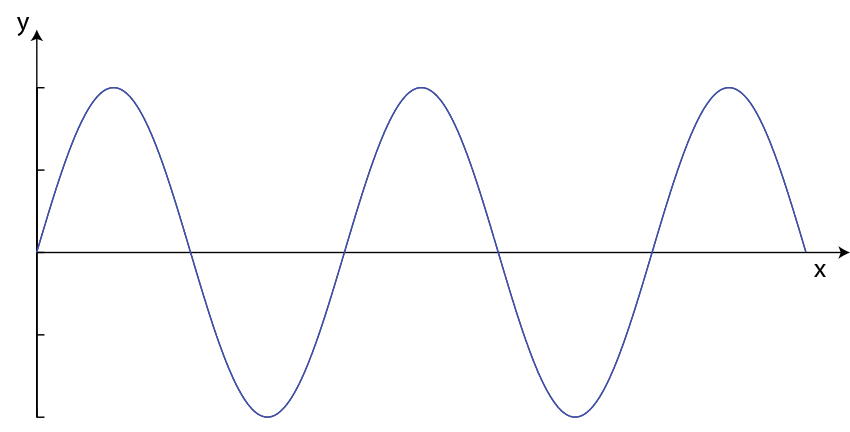
\includegraphics[width=7.2cm]{images/sine3.png}
	}
	\subfloat[Value- and time-discrete signal.]{
		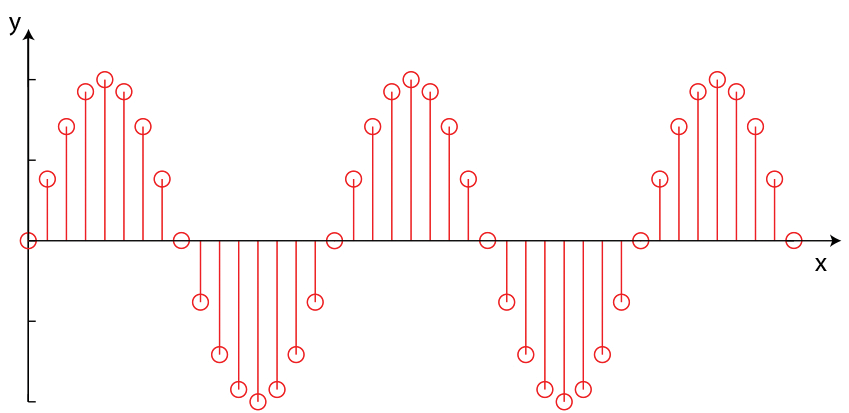
\includegraphics[width=7.2cm]{images/sine4.png}
	}
	\caption{
		Quantization.
	}
	\label{fig:quantization}
\end{figure}

The sampling creates the time discrete signal. Thereby, the sampling rate $f_s$, which is the number of frames per seconds (fps) in the digital signal, is specified in Hz. Typical sampling rates are 8000 Hz, 22.000 Hz or 44.100 Hz. A frame is also called \textit{sample}. To receive a good sampling rate, the sampling theorem, which is described in \autocite{Zoelzer:2008}, needs to be considered. In general, a fast varying signal has to be sampled higher than a slowly varying one. This way, the original signal can be represented with a reasonable degree of accuracy.
%Sampling Theorem Walter seite 56!
% Eine sinnvolle zeitliche Diskretisierung liegt vor, wenn die Veränderungen des analogen Signals durch die Abtastfolge gut wiedergegeben werden. Damit das analoge Signal aus der Abtastfolge durch eine Interpolation hinreichend genau wieder gewonnen werden kann, muss ein sich schnell änderndes Signal häufiger als ein dazu relativ langsam veränderliches Signal abgetastet werden. Diese grundsätzliche Überlegung wird im Abtasttheorem präzisiert.

The quantization displays the signal amplitudes by a given bit rate. By default, a bit rate of 8 bit or 16 bit is used. This procedure is performed by an analog to digital converter. 

Further information about sampling and quantization of analog signals can be found in \autocite{Werner:2012} and \autocite{Zoelzer:2008}.

\subsection{Frequency Spectrum Analysis of Digital Signals} 
For this thesis, the most important signal processing method is the conversion of a digital audio signal to its frequency spectrum. This spectrum displays the distribution of energy within the frequency domain. 

The frequency domain of a digital signal is affected by sampling and sampling rate. If an analog signal is sampled with a sampling rate of 40100 Hz, the frequency range from 0 Hz up to 20050 Hz $($half of the sampling rate$)$ is mirrored between 20000 Hz and 40100 Hz. The amplitudes between 0 Hz and 20050 Hz are the same in both spectra. The effect is shown in figure \ref{fig:analogDigitalSpectra}. 

% The sampling operation leads to a replication of the baseband spectrum of the analog signal [Orf96]. The frequency contents from 0 Hz up to 20 kHz of the analog signal now also appear from 40 kHz up to 60 kHz and the folded version of it from 40 kHz down to 20 kHz. The replication of this first image of the baseband spectrum at 40 kHz will now also appear at integer multiples of the sampling frequency of fs = 40 kHz. But notice that the spectrum of the digital signal from 0 up to 20 kHz shows exactly the same shape as the spectrum of the analog signal. The reconstruction of the analog signal out of the digital signal is achieved by simply lowpass filtering the digital signal, rejecting frequencies higher than f s / 2 = 20 kHz.

% zoelzer figure 1.5
\begin{figure}[h]
	\centering
	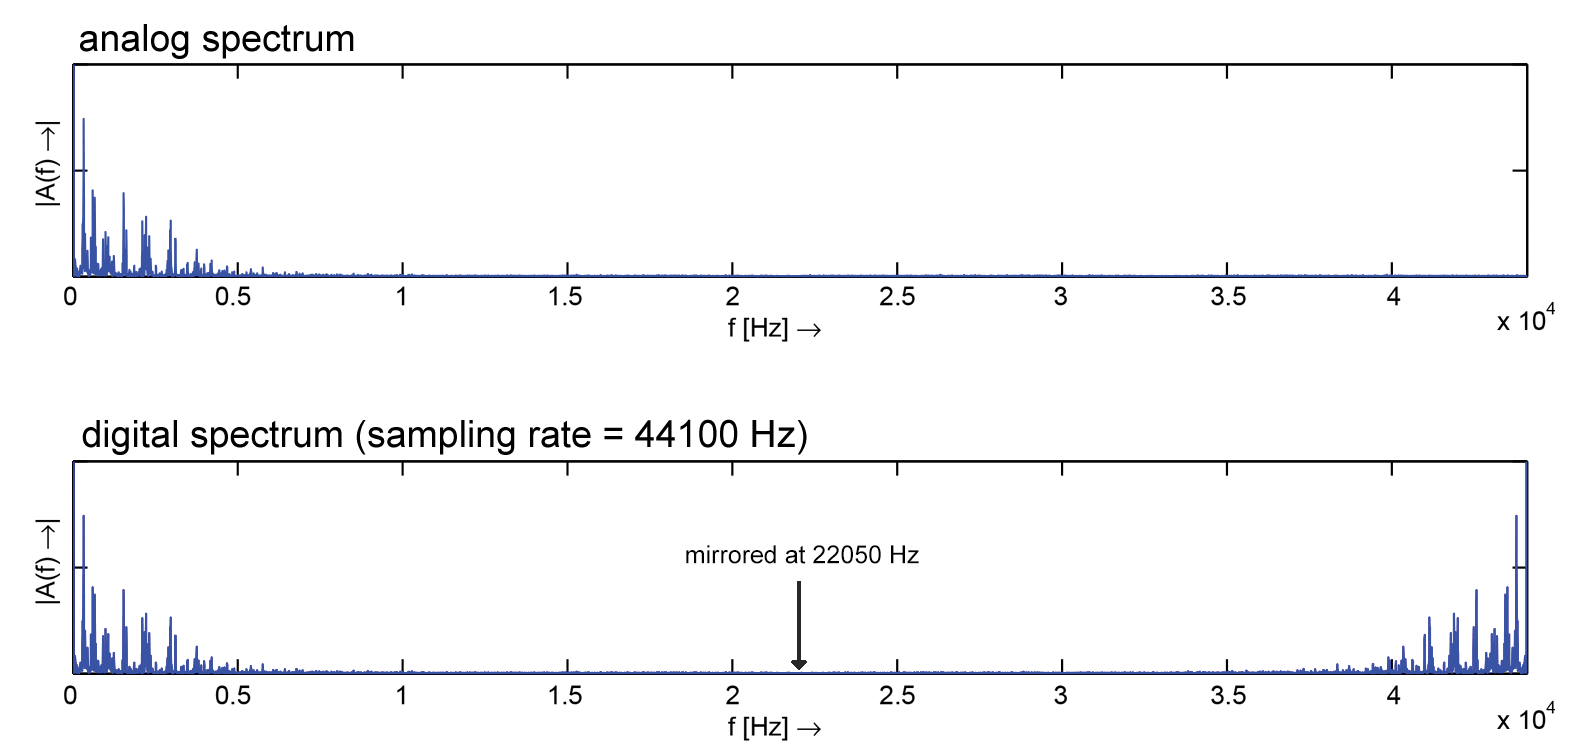
\includegraphics{images/analogDigitalSpectra.png}
	%for reference to this figure
	\caption{ Spectra of analog and digital signals.}
	\label{fig:analogDigitalSpectra}
\end{figure}

\subsubsection{Discrete Fourier Transformation}

To decompose the time series $x[n]$ of an audio signal into its frequency spectrum $X[k]$, the Fourier series and the Fourier transform are fundamental methods. They are based on the research of Jean Baptiste Joseph Fourier in the 18th century. The Fourier series is used to convert periodic time continuous signals and the Fourier transform is used to convert aperiodic time continuous signals. Based on the Fourier series, the \textit{Discrete Fourier Transform (DFT)} can be used on time discrete periodic signals. In contrast to the Fourier transform or Fourier series, the DFT can be used for short time spectral analysis, which is described in section \ref{section:shortTime} \autocite[]{Werner:2012}.


In \autocite[]{Zoelzer:2002} the DFT is defined as a series of DFT-coefficients by

\begin{equation}
X(k)=DFT[x(n)]=\sum_{n=0}^{N-1}x(n)e^{-j2\pi nk/N}, k=0,1,2,...,N-1
\label{equation:DFT}
\end{equation}

\subsubsection{Short Time Spectral Analysis and Windowing} \label{section:shortTime}

A short time spectral analysis is a spectral analysis which is only applied to short blocks of a signal. These blocks are called \textit{windows}. The DFT allows it to be used block oriented because of its periodic exponential function $exp(-j2\pi nk/N)$, which is described in equation \ref{equation:DFT}. It assigns to N elements of a periodic signal exactly N frequency bins in the resulting spectrum. Thus, the larger the window is, the higher the resolution of the resulting frequency spectrum.

In real-time audio processing the incoming signal is divided into a sequence of windows. They can be abutting or overlapping \autocite[]{Werner:2012}.

The DFT assumes that the signal is continued periodically. Hence, for a periodic signal, the window size should be a minimum of an entire period because otherwise there is a loss of information. Further on, as an optimum, the window should begin at the same point in the period as it ends. But this is not possible for audio signals because they are usually not periodic. In this case, not existing spectral components can appear in the frequency domain. This type of occurrences is called \textit{leakage phenomenon} \autocite[]{Werner:2012}.

To reduce the effect of the leakage phenomenon, the form of the window can be changed by applying a so called window function. Thereby, the wave is flattened in its beginning and end. If a window with window function is periodically continued, there is no more leap in the wave. The effect is shown in figure \ref{fig:window1}.

\begin{figure}[h]
	\centering
	\subfloat[Without window function.]{
		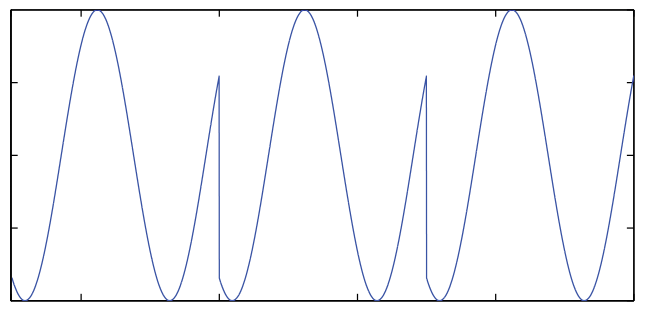
\includegraphics[width=7.2cm]{images/sine5.png}
	}
	\subfloat[With window function (Hamming window).]{
		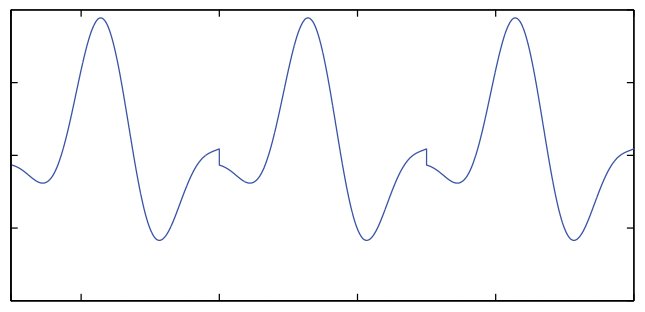
\includegraphics[width=7.2cm]{images/sine6.png}
	}
	%for reference to this figure
	\caption{ Periodically repeated window of values. }
	\label{fig:window1}
\end{figure}

Common window functions in the field of audio processing are the Hamming Window or the Hanning Window. These and other window functions are explained in \autocite[]{Harris:1978}. Figure \ref{fig:window2} shows some common functions.

\begin{figure}[h]
	\centering
	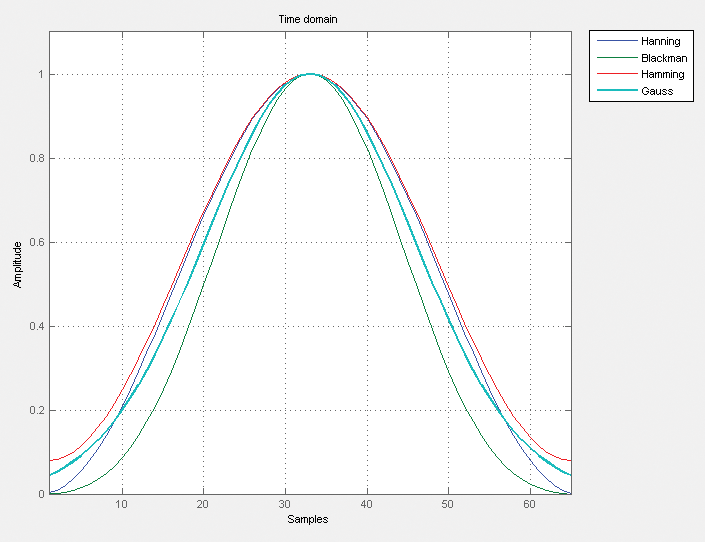
\includegraphics[width=11cm]{images/windowfunctions.png}
	%for reference to this figure
	\caption{Window functions.}
	\label{fig:window2}
\end{figure}

\subsubsection{Fast Fourier Transformation}
The \textit{Fast Fourier Transformation (FFT)} is an efficient version of the DFT. There are many different approaches for FFT algorithms, today. They are based on the fact that a series of real number x[n] with an even length $N=2M$ can be decomposed to a complex series of half the length of N. Thus, the DFT can be decomposed in two parts - one with even and one with odd indices. One of the most popular FFT algorithms is the Radix-2-FFT. The complexity of the direct use of the DFT is $O(N^2)$, whereas the Radix-2-FFT has a complexity of $O(N log_2(N))$. Hence, the FFT allows to use digital signal processing in real-time. 

% Fourier Analysis can be used to identify naturally occurring harmonics (which are, simply put, the basis of all musical composition), to model sound, and to break up sound into the pieces that define it.

% The spectrumo f a digital signal can be computedb y the discrete Fourier transform DFT which is given by
% (1.1)
% The fast version of the above formula is called the fast Fourier transform FFT. The FFT takes N consecutive samples out of the signal z(n) and performs a mathematical operation to yield N sa,mples X ( k ) of the spectrum of the signal. Figure 1.6 demonstrates the results of a, 16-point FFT applied to 16 samples of a cosine signal. The result is normalized by N according to X=abs (fft (x ,N) ) /N; .
% The N samples X ( k ) = X,(k) + j X l ( k ) are complex-valued with a real part XR(IC) and an imaginary parXt ~ ( l cf)ro m which one can compute the absolutvea lue
% (1.2)
% which is the magnitude spectrum, and the phase
% (1.3)
% which is the phase spectrum.

% Frequency Resolution: Zero-padding and Window Functions
% To increase the frequency resolution for spectrum analysis we simply take more samples for the FFT algorithm. Typical numbers for the FFT resolution are N = 256,512,1024,2048,4096 and8 192. If we are only interested in computing thes pectrum of 64 samples and would like to increase the frequency resolution from f,/64 to f,/1024, we have to extend the sequence of 64 audio samples by adding zero samples up to the length 1024 and then performing an 1024-point FFT. This technique is called zero-paddingand is illustrated in Fig. 1.8 and by M-file 1.5. The upper left part shows the original sequence of 8 samples and the upper right part shows the corresponding 8-point FFT result. The lower left part illustrates the adding of 8 zero samples to the original 8 sample sequence up to the length of N = 16. The lower right part illustrates the magnitude spectrum IX(k)l resulting from the 16-point FFT of the zero-padded sequence of length N = 16. Notice the increase in frequency resolution between the 8-point and 16-point FFT. Between each frequency bin of the upper spectrum a new frequency bin in the lower spectrum is calculated. Bins k = 0,2,4,6,8,10,12,14 of the 16-point FFT correspond to bins k = 0,1,2,3,4,5,6,7 of the 8-point FFT. These N frequency bins cover the frequency range from 0 Hz up to v fs Hz.



\subsection{Onset Detection} \label{section:OnsetDetection}

Before a drum stroke can be analyzed it has to be found in the signal stream. For this, onset detection is used. There are many different methods of onset detection right now. \autocite{Bello:2005} describes some important ones. The paper focuses on note onset detection in musical signals.

The audio signal that describes a single note can be divided into several parts. As shown in figure \ref{fig:OnsetDetection1}, \autocite{Bello:2005} differentiates between \textit{onset}, \textit{attack}, \textit{transient} and \textit{decay}. The onset is defined as the point in time, where the wave shows the first signs of a new note. The attack is the interval after an onset, where the amplitude is rising. The transient describes the part of the wave, where the signal evolves. In case of a drum stroke, this would be the time from the first contact of the drum stick on a drumhead until the sound is damped by the stroke. Subsequently, the sound decays. In \autocite{Bello:2005} it is assumed that the human ear cannot distinguish between two transients less than 10 ms apart.

\begin{figure}[h]
	\centering
	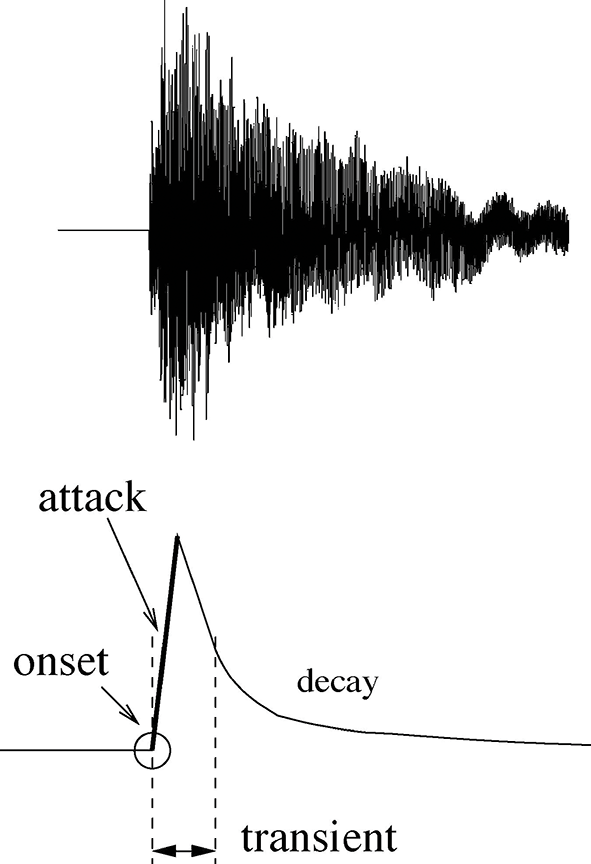
\includegraphics[width=4.0cm]{images/bello_2005_Seite_01_Bild_0001.png}
	\caption{Attack, transient, decay and onset of a sound \autocite[Fig. 1]{Bello:2005}.}
	\label{fig:OnsetDetection1}
\end{figure}

Most onset detection algorithms consist of three steps, like shown in figure \ref{fig:OnsetDetection2}. In the first step, which is optional, the original signal is pre-processed to achieve a better performance in the further steps. Example methods are to separate the signal into multiple frequency bands or to use transient/steady-state separation. The second step is the reduction of the pre-processed audio signal. The reduction is the key process in onset detection. Here, a detection function is created to which a peak picking algorithm can be applied in the last step. These peaks represent the points in time of all onsets in the original audio signal. 

In \autocite[]{Bello:2005} a couple of common onset detection algorithmse are introduced. The paper explains reduction methods based on a signal's amplitude envelope, spectral magnitudes and phases, time-frequency representation and methods based on probabilistic signal models. A basic method that considers the amplitude envelope of audio signals is shown in \autocite[]{Schloss:1985}. It is explained in section \ref{section:OnsetDetectionSchloss}.

\begin{figure}[h]
	\centering
	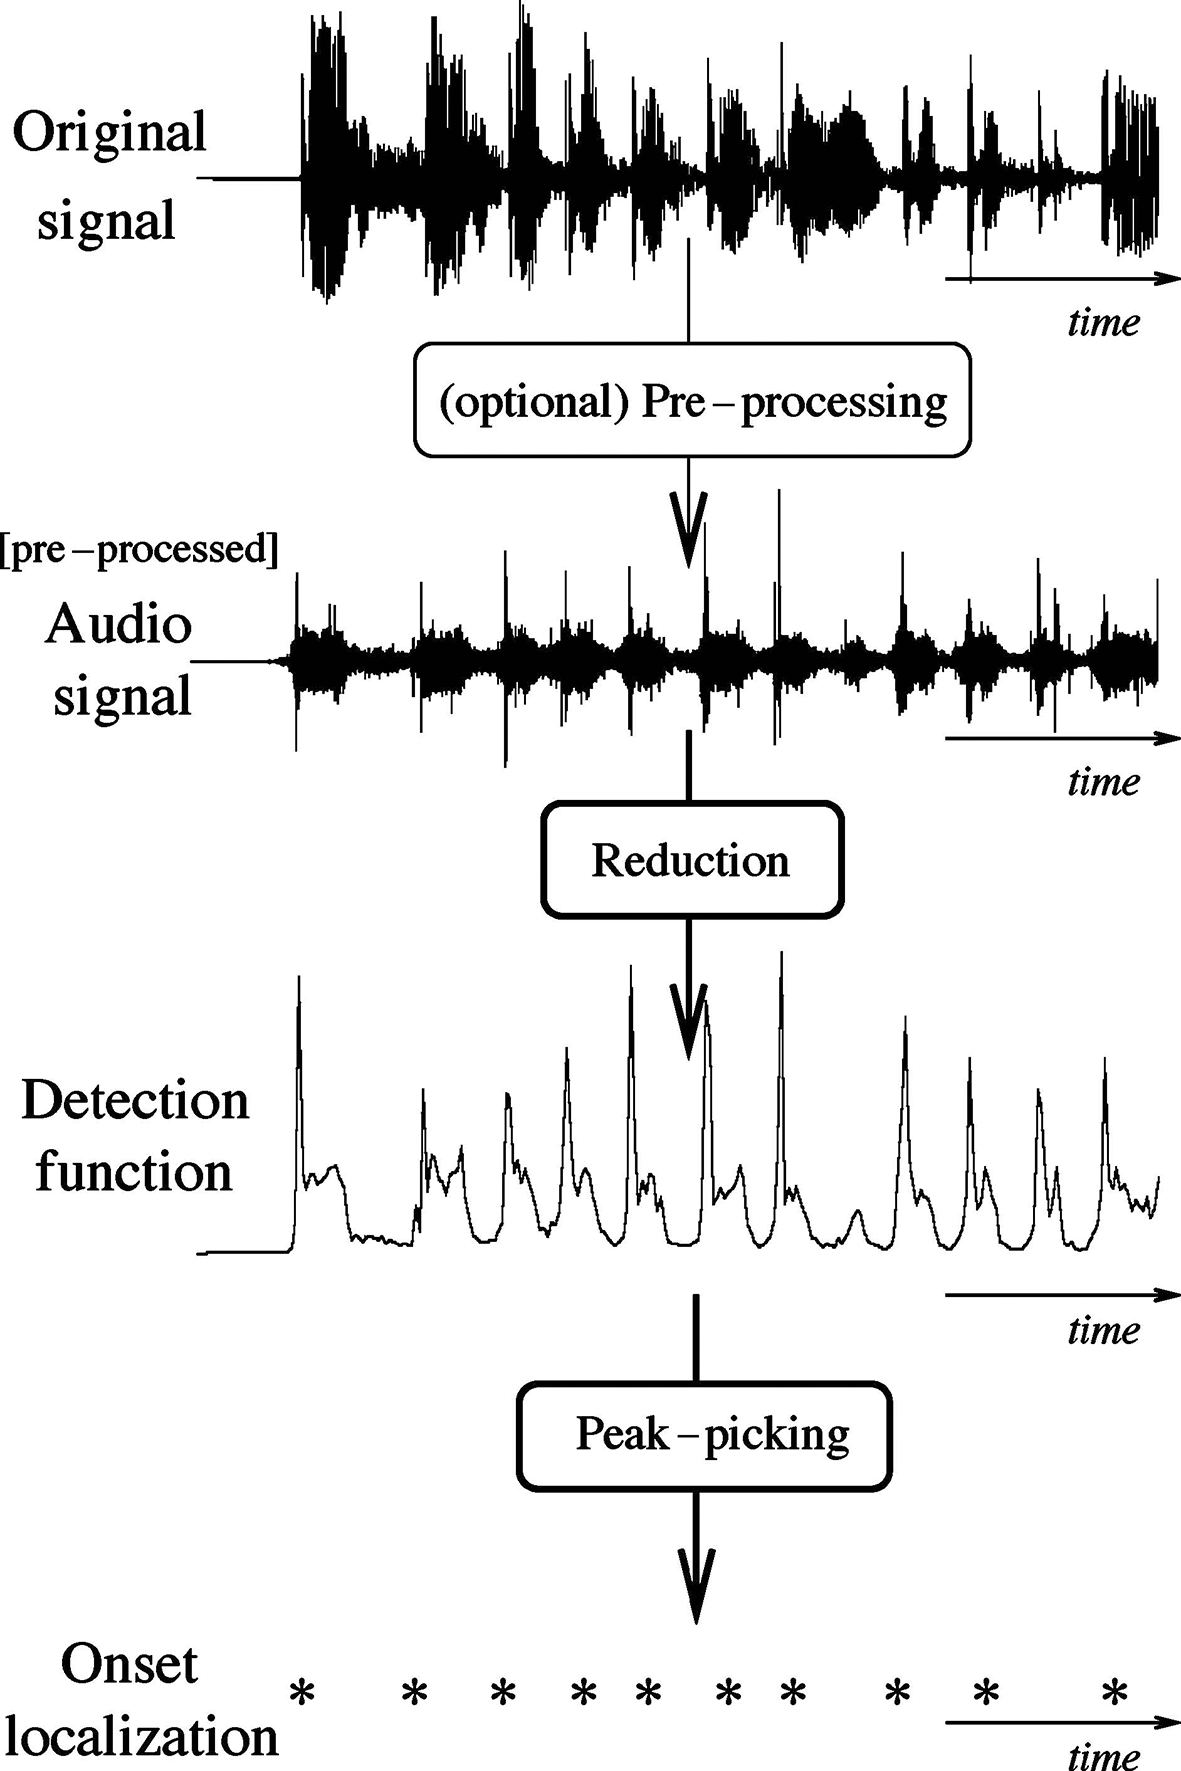
\includegraphics[width=7.0cm]{images/bello_2005_Seite_02_Bild_0001.png}
	\caption{Flowchart of a standard onset detection algorithm \autocite[Fig. 2]{Bello:2005}.}
	\label{fig:OnsetDetection2}
\end{figure}



\subsection{Classification}

After the detection of an onset, the proximate audio information can be classified as one of the drums of the used drum set. Therefore, a classification algorithm is needed. 

Classification describes the attempt to determine class labels for data instances by the use of training data. This process is called \textit{supervised learning}, in contrast to the field of clustering, where \textit{unsupervised learning} is used. A detailed introduction to data classification algorithms and applications can be found in \autocite{Chapman:2015}. There are various different approaches for the classification of data for widespread subjects in computer science.

Generally, a classification algorithm is divided into two steps. The first is the \textit{training} in which a model is built with the help of a training set. The training set contains several labeled data of each possible instance. The second step is the \textit{testing}, where the model is used to assign a label to a test instance. There are also some methods without training. Here, testing refers directly to the training data, which is described as \textit{lazy leaning}. The output of the classification algorithm can be either a discrete label or a numerical score for each possible class.

There are various numbers of classification methods used for different data types. Common data types are text data, multimedia data, uncertain data, time series or discrete sequences. In this thesis audio signals are considers, which is continuous multimedia data. Furthermore, as a main part of the thesis, the frequency spectra of the audio data are used to classify the signals. A frequency spectrum is a sequence, which means a finite, ordered number of values. To classify sequential data, \autocite{Chapman:2015} proposes feature based, distance based and model based classification methods. The general procedure for multimedia data learning is explained by figure \ref{fig:datalearning}. It persists of four steps, which are the preparation of the data, the data pre-processing and feature extraction, the model learning and finally the prediction of unknown data instances.

\begin{figure}[h]
	\centering
	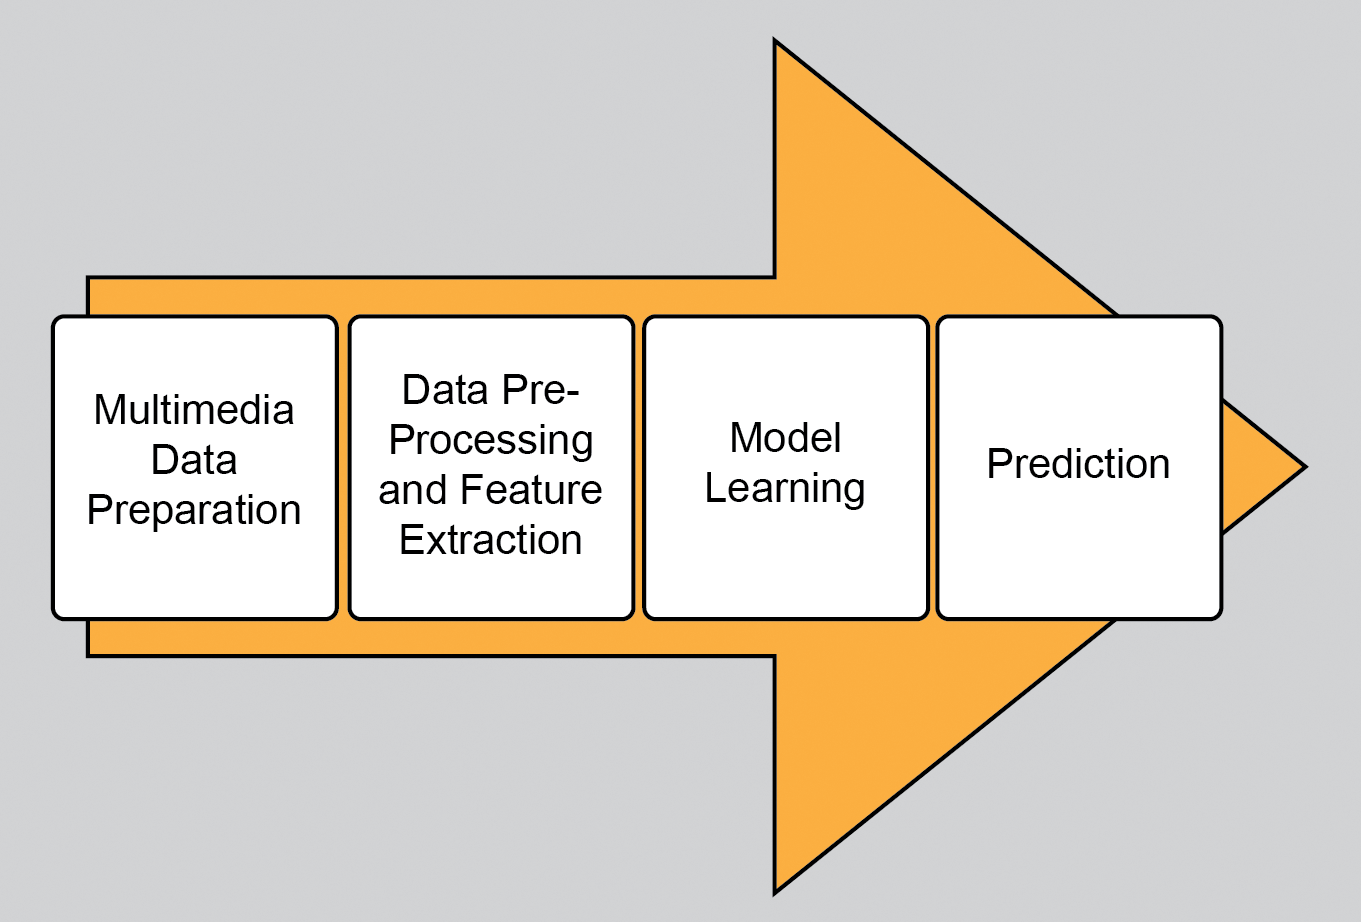
\includegraphics[width=8.0cm]{images/datalearning.png}
	\caption{Flowchart of general multimedia learning process. \autocite[Fig. 12.1]{Chapman:2015}.}
	\label{fig:datalearning}
\end{figure}

\subsubsection{Feature Extraction}

The deciding step in the data classification process is a reasonable data pre-processing and feature extraction. By the extraction of significant features, the model learning and prediction can turn into trivial problems. On the contrary, insignificant features can adulterate the classification result, especially when a small training set is used. As an example, \autocite{Chapman:2015} shows two speech sequences which contain the same sentence spoken by different persons. The resulting waveforms in the time domain are very different and can hardly be assigned as the same sentence. But if the same data is transformed to its frequencies over time, the resulting charts are largely the same. Thus, all used features need to be analyzed in detail.

%\begin{figure}[h]
	%\centering
	%\includegraphics[height=8.0cm]{images/classification/speechexample1.jpg}
	%\caption{Time domain waveform of the same spoken sentence from different persons. \autocite[Fig. 12.2]{chapman:2015}.}
	%\label{fig:speechexample1}
%\end{figure}
%\begin{figure}[h]
	%\centering
	%\includegraphics[height=8.0cm]{images/classification/speechexample2.jpg}
	%\caption{Frequencies over time of the speech in figure \ref{fig:speechexample1} \autocite[Fig. 12.3]{chapman:2015}.}
	%\label{fig:speechexample2}
%\end{figure}

%\subsubsection{Feature Extraction}
%Before the classification is executed, it is important to create a significant feature vector. This vector should only contain values which describe the properties of the classes. Insignificant features can adulterate the classification result, especially when a small training set is used. Using the example of drum sound classification such a feature could be the volume of a drum stroke. If one drum instance has more training data with a higher volume than a second one, all drum with a high volume will be classified as the first drum. Thus all used features has to be analyzed in detail.

For audio data, three different groups of frequently used features can be summarized. These are time domain features, frequency domain features and psycho acoustic features. The latter mainly consider classification of data containing speech and thus irrelevant for this thesis. In time domain, there can be extracted features based on the energy of the audio waveform or the so called zero crossing rate, which counts the number of times the waves goes trough the zero axis within a frame. In the frequency domain an often used feature is the pitch, which defines the fundamental frequency of an audio signal. Subband energy ratios showing the distribution of energy over a predefined frequency band can also be considered. Additionally, there are several methods to extract values based on spectral statistics, like frequency centroids and bandwidth. 

\subsubsection{Feature Based Classification}

The extracted features are usually combined to a feature vector that is used to train a classification model. Thereby, each feature vector represents one of the used class labels. Afterward, new data instances can be predicted with the help of this model. Therefore, the same feature vector needs to be build for the new data. As already mentioned in the preceding section, meaningful features need to be chosen to ensure a high hit-rate for correctly classified instances. Further on, there should not be too many features because the complexity rises with more features for the most classification methods. For feature based classification, common methods are decision trees or statistical methods like naive Bayes, which builds a probabilistic model. In this thesis, decision trees will be used in section \ref{section:method1}. Hence, a short introduction to decision trees is given in the following section.

%Bayesian Classification
%The Bayesian Classification represents a supervised learning method as well as a statistical method for classification. Assumes an underlying probabilistic model and it allows us to capture uncertainty about the model in a principled way by determining probabilities of the outcomes. It can solve diagnostic and predictive problems. 
%This Classification is named after Thomas Bayes ( 1702-1761), who proposed the Bayes Theorem. 
%Bayesian classification provides practical learning algorithms and prior knowledge and observed data can be combined. Bayesian Classification provides a useful perspective for understanding and evaluating many learning algorithms. It calculates explicit probabilities for hypothesis and it is robust to noise in input data.
% decision trees used for this thesis in ... , explained in the following section.

\subsubsection{Decision Trees} 
%introduction to decision trees

One of the most common classification algorithms for solving complex decision-making tasks based on a feature vector is the decision tree. In contrast to other algorithms it's structure is very comprehensible and intuitive for users. An introduction to decision trees is given in \autocite{Chapman:2015}. The decision tree is a rooted, directed tree, which builds a hierarchical structure of conditions. To construct the tree, the extracted feature vectors for every training data instance are passed on to the training algorithm with its appropriate class labels. This training algorithm is called \textit{decision tree induction}. The classical approach for decision tree induction is the top-down selection of partitioning rules on a static data set. It is described in \autocite{Chapman:2015}. After building the tree, it can be used as a classification function to label unseen data instances. 

Every decision tree contains nodes that describe conditions called \textit{splitting rules}. The splitting rules divide the data into separated classes by using the attributes of the feature vector. Most algorithms use one attribute, thus one condition, for each node. The resulting splitting rules are called \textit{univariate}. Some algorithms also use multiple attributes in one node called \textit{multivariate} splitting rules. Furthermore, there are \textit{binary decision trees} and trees with \textit{multiway splits}. In this thesis, binary decision trees are considered. Thus, each node in the tree that is no leaf node has two child nodes.
%Many decision trees are binary, with each partitioning rule dividing its subspace into two parts. Even binary trees can be used to choose among several class labels. Multiway splits are also common, but if the partitioning is into more than a handful of subdivisions, then both the interpretability and the stability of the tree suffers.

To classify an unseen data instance, it passes the nodes by following their splitting rules, beginning at the root node. Thus, each condition in a splitting rule decides to which child node the data instance is going to be transmitted. The process stops when a leaf of the tree is reached. Each leaf node represents a class label.

In most cases, the aim of the decision tree algorithm is not only to find a model that classifies all instances correctly, but also to build a system with a good complexity. The complexity of a decision tree can be measured by the total number of nodes, the total number of leaves, the depth of the tree and the number of attributes used by the splitting rules. To reduce the complexity a method called \textit{pruning} is used, which reduces the depth of the tree \autocite{Bhargava:2013}. This way, the calculation time can be decreased, whereupon the accuracy of the classification may suffer. Thus, a compromise of accuracy and complexity needs to be found.
%{chapman:2015} Ideally, we would like a method with fast tree construction, fast predictions (shallow tree depth), accurate predictions, and robustness with respect to noise, missing values, or concept drift.
%{chapman:2015} The number of possible trees grows exponentially with the number of attributes and with the number of distinct values for each attribute

\begin{table}[htb]
  \caption{Example: Contact Lens Recommendations \autocite{Chapman:2015}}
  \label{tab:c45trainingset} 
	\centering
	\footnotesize
	\begin{tabular}[c]{|c|c|c|c|c|}
	  \hline
		\textbf{Age}	&	\textbf{Near-/Far-sightedness}	&	\textbf{Astigmatic}	&	\textbf{Tears}	&	\textbf{Contacts Recommended} \\
		\hline \hline
		13	&	nearsighted	&	no	&	reduced	&	no \\
		\hline
		18	&	nearsighted	&	no	&	normal	&	yes \\
		\hline
		14	&	nearsighted	&	yes	&	reduced	&	no \\
		\hline
		16	&	nearsighted	&	yes	&	normal	&	yes \\
		\hline
		11	&	farsighted	&	no	&	reduced	&	no \\
		\hline
		18	&	farsighted	&	no	&	normal	&	yes \\
		\hline
		8	&	farsighted	&	yes	&	reduced	&	no \\
		\hline
		8	&	farsighted	&	yes	&	normal	&	yes \\
		\hline
		26	&	nearsighted	&	no	&	reduced	&	no \\
		\hline
		35	&	nearsighted	&	no	&	normal	&	yes \\
		\hline
		39	&	nearsighted	&	yes	&	reduced	&	no \\
		\hline
		23	&	nearsighted	&	yes	&	normal	&	yes \\
		\hline
		23	&	farsighted	&	no	&	reduced	&	no \\
		\hline
		36	&	farsighted	&	no	&	normal	&	yes \\
		\hline
		35	&	farsighted	&	yes	&	reduced	&	no \\
		\hline
		32	&	farsighted	&	yes	&	normal	&	no \\
		\hline
		55	&	nearsighted	&	no	&	reduced	&	no \\
		\hline
		64	&	nearsighted	&	no	&	normal	&	no \\
		\hline
		63	&	nearsighted	&	yes	&	reduced	&	no \\
		\hline
		51	&	nearsighted	&	yes	&	normal	&	yes \\
		\hline
		47	&	farsighted	&	no	&	reduced	&	no \\
		\hline
		44	&	farsighted	&	no	&	normal	&	yes \\
		\hline
		52	&	farsighted	&	yes	&	reduced	&	no \\
		\hline
		46	&	farsighted	&	yes	&	normal	&	no \\
	  \hline
	\end{tabular}
\end{table}

\begin{figure}[htb]
	\centering
	\subfloat[Unpruned tree.]{
		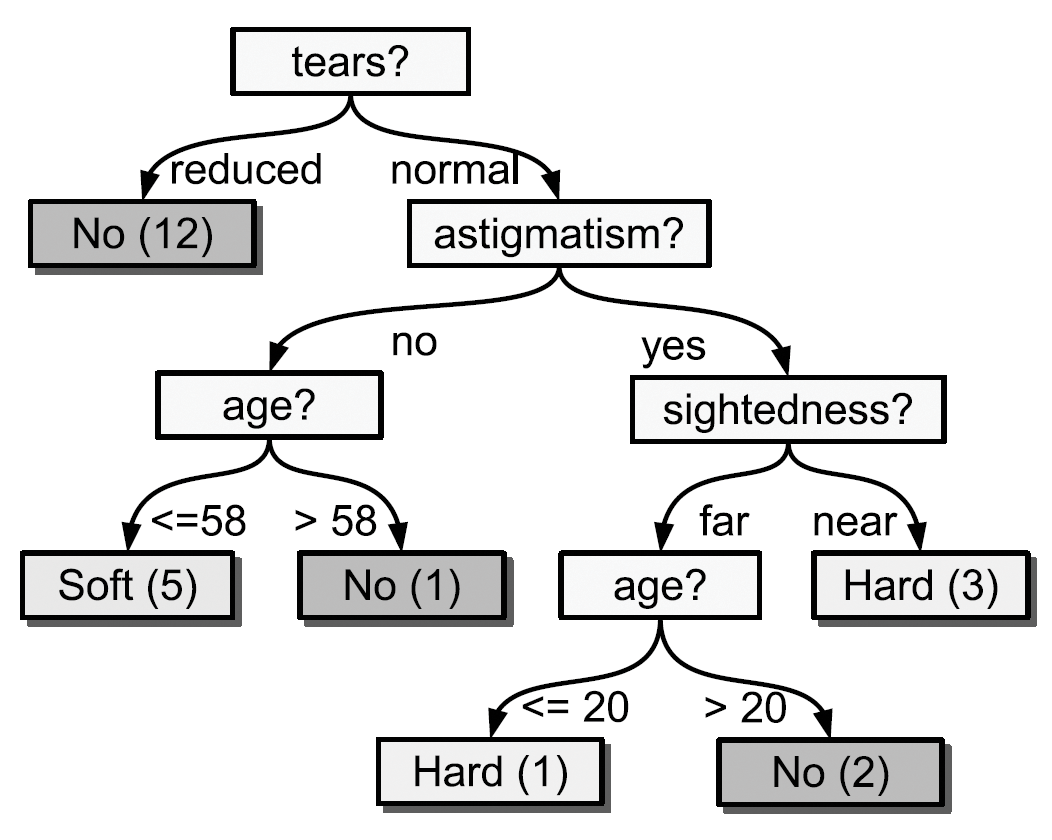
\includegraphics[height=5.0cm]{images/exampletree1.png}
		\label{fig:exampletree1}
	}
	\qquad
	\subfloat[Pruned tree.]{
		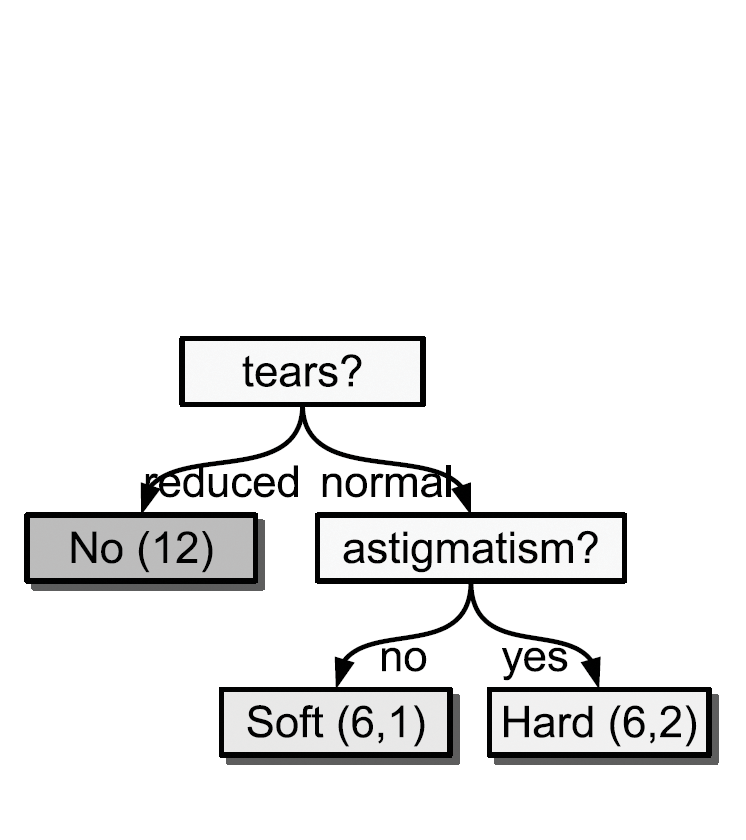
\includegraphics[height=5.0cm]{images/exampletree2.png}
		\label{fig:exampletree2}
	}
	\caption{
		C4.5 decision tree \autocite[Fig. 4.2]{Chapman:2015}
	}
	\label{fig:exampletree}
\end{figure}

For this thesis we will use a C4.5 tree that uses the J48 algorithm. A sample C4.5 decision tree is shown in figure \ref{fig:exampletree}. This tree helps to decide whether a person can wear contact lenses or not. The training set which is used to build the tree is displayed in table \ref{tab:c45trainingset}. Each data record contains information about a person. They include the age of the person as a numerical value and three Boolean values, which are `Near-/Far-sightedness', `Astigmatic' and `Tears'. The last value in the table defines the appropriate class label, which can be `yes' or `no'. The example is taken from \autocite{Chapman:2015}. Figure \ref{fig:exampletree1} shows an unpruned tree that labels all instances correctly. It has a total number of eleven nodes, six leafs and a maximum depth of five. The pruned version of the tree displayed in figure \ref{fig:exampletree2} has only three nodes, two leafs and a depth of two, but labels three instances incorrectly.

\subsubsection{Further Classification Methods}

Next to the feature based methods described in the preceding, there are several other approaches for data classification. In \autocite{Chapman:2015}, distance based and model based methods, which can be used to classify data sequences, are introduced as well.

Distance based classification methods use the distance between two sequences to label unseen data instances. An example for a distance based classification method is the \textit{k-NN (nearest neighbors)} classifier that uses lazy learning. It calculates the distance to all training data to find the nearest neighbor for an unseen data instance. Another common classification system, which uses the similarity instead of the distance between data instances, is the \textit{support vector machine (SVM)}. It calculates the similarity by the construction of a so called \textit{kernel function}. The \textit{SVM} is used in multiple cases to classify audio data.

Model based classification methods build a probabilistic model for each possible class label. These models are used to label unseen data instances. Therefore, a probabilistic function like Bayes rule is used. For each trained class, the probability  is returned that the new data instance is built with the appropriate model. A sample algorithm used to build probabilistic models is the Hidden Markov Model (HMM). It is used by \autocite{Simsekli:2011} for the real-time classification of drum sound, which is described in section \ref{section:realtimeapproach}.

\subsubsection{Evaluation}

To assert the accuracy of a classification algorithm, it needs to be evaluated. Thereby, it has to be regarded that the used test data is not part of the data used to train the system before. Thus, some labeled instances have to be removed before training. There are several methods to do this, such as \textit{hold out} or \textit{cross-validation}. The \textit{hold out} method is the simplest one. Here, a predefined percentage of labeled instances is removed for training and used for testing. In \textit{cross-validation}, the training set is divided into k disjoint subsets. One of the subsets is used for testing, the remaining ones for training. The procedure is repeated k times, so every subset is used for testing, once. This method ensures that every labeled instance is used for training and testing without using trained instances in the test phase.


\subsection{Tools}

To develop and test the algorithms presented in this thesis, MatLab\textsuperscript{\textregistered} and Weka are used as tools.

\subsubsection{MatLab\textsuperscript{\textregistered}}
To extract features of a sound, multiple signal processing methods are necessary. Therefore, MatLab\textsuperscript{\textregistered} \autocite{MathWorks:2014} can be used. MatLab\textsuperscript{\textregistered} is a programming language and interactive environment for numerical computation, visualization, and programming. It provides several built-in function and extension packages for a widespread application range, such as signal processing and communication, image and video processing, control systems, test and measurement, computational finance, and computational biology. For audio processing purposes, it contains a signal processing toolbox that includes several functions, like FFT or window functions. Hence, MatLab\textsuperscript{\textregistered} allows a fast development of new algorithms and can be used to analyze data. In this thesis it is used to develop the onset detection and classification methods and to visualize and evaluate the gained results.

\subsubsection{Weka}

Next to MatLab\textsuperscript{\textregistered}, the data mining tool \textit{Weka} developed by the University of Waikato \autocite{Weka:2014} is used to test and evaluate classification algorithms. Weka contains several machine learning algorithms, such as tools for data pre-processing, classification, regression, clustering, association rules, and visualization. Furthermore, it gives an evaluation overview after each test. A sample output is shown in figure \ref{fig:weka}. Here, a test set with four different drums is used with the Naive Bayes classifier. The labeled data input contains 140 instances and four attributes. It is divided into a training set and a test set with a percentage split of 50 \%. The Weka output gives a detailed overview on the Naive Bayes specific classification results and the time taken to build the model. In the example the time is 0.02 seconds. Further on, the evaluation of the test split is listed. There are 97.15 \% correctly classified and 2.85 \% incorrectly classified instances. The total number of tested instances is 70, whereof 68 instances are correctly classified. Moreover, there is a table showing the detailed accuracy by class and a confusion matrix. The confusion matrix shows as which class the instances are classified. In the example, two instances are classified incorrectly. One with the label `bass' is classified as `tom3' and one with the label `snare' is classified as `tom2'.

\begin{figure}[h]
	\centering
	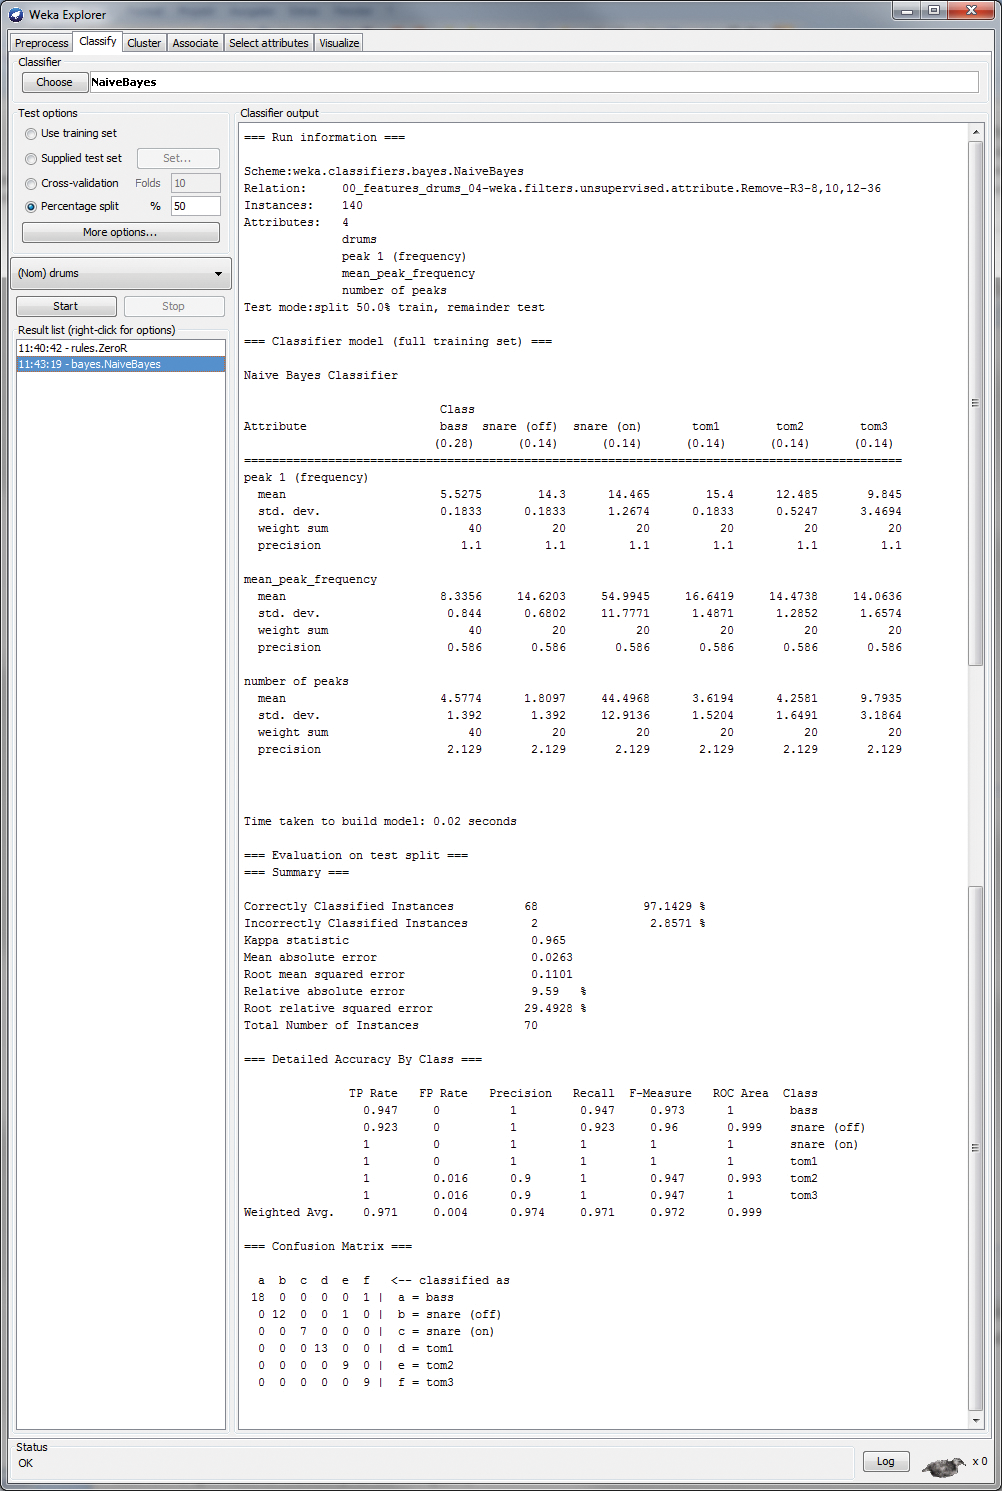
\includegraphics[height=16cm]{images/weka.png}
	\caption{Example Weka output of Naive Bayes classification algorithm for different drum types}
	\label{fig:weka}
\end{figure}


\subsection{Audio Processing in the Web}

As described in section \ref{section:Easydrum}, the aim of this thesis is to develop a listener component for the platform Easydrum, which is able to receive played drum sounds by the audio input through a connected microphone. This listener has to map the incoming sound to the appropriate drums and cymbals and further to save the points in time when a stroke was performed. To realize this, the incoming audio data has to be processed with the help of JavaScript. The data need to be analyzed to find the onsets of performed strokes and to classify these strokes. Hence, a web technology is needed that is able to process audio data.

The actual web standard for the handling of audio data in the web is limited to the \lstinline{<audio>} object of the Audio Data API. These object provides the functionality of playing and get limited information about audio data, but does not enable editing or creation of data. Other limited technologies used to access audio information in recent web applications are Flash or the QuickTime plug-in. However, Easydrum tries to use modern web technologies and thus wants to operate without Flash and QuickTime. As described in section \ref{section:Easydrum}, it uses the Web Midi Api \autocite{WebMidiApi:2015} to receive MIDI input in the browser. This API is not yet a standard but is already largely accessible with the Google Chrome browser and can be simulated in other browsers with the help of the JazzPlugin \autocite{JazzPlugin:2015}.

Concurrently with the Web Midi API, the W3C has been developing the Web Audio API, which is specified by the Audio Working Group as an Editor's Draft \autocite{WebAudioApi:2015}. It is a high-level JavaScript API for processing and synthesizing audio data in web applications. It offers the possibility to create interactive applications with audio content just as audio recorder, sequencers or games with audio content. It can receive audio data from input devices, process them and send them to output devices. This procedure is realized via the provided audio context, which contains different audio processing modules. To process audio operations, audio nodes are used inside the audio context. Different audio nodes can be linked together by their inputs and outputs to form an audio routing graph. According to \autocite{WebMidiApiMDN:2015}, the timing of the Web Audio API `is controlled with high precision and low latency, allowing developers to write code that responds accurately to events and is able to target specific samples, even at a high sample rate.' Additionally, it can be used with the canvas 2D of HTML 5, which is used by Easydrum. Like the Web Midi API, the functionality of the Web Audio API is already largely accessible in the Google Chrome browser. The main methods of the API are also implemented in Firefox since version 25. For browsers that don't support the Web Audio API, there are different JavaScript libraries that provide different fallback solutions to the Audio Data API or to Flash. An example for a library is WAAPISim \autocite{WAAPISim:2015}.

Next to processing audio data, it is required for the Easydrum extension to get access to a microphones input data. This functionality is provided by the WebRTC, which has been developed for the real-time communication between browsers. It is able to receive video and audio streams from local devices like web cams and microphones. The received audio stream can be processed by the Web Audio Api. The WebRTC version 1.0 was published as a working draft \autocite{WebRTC:2015}. 

Hence, the Web Audio API combined with the WebRTC provides the required functionality for the Easydrum extension developed in this thesis.

%An AudioBuffer takes as its parameters a number of channels (1 for mono, 2 for stereo, etc), a length, meaning the number of sample frames inside the buffer, and a sample rate, which is the number of sample frames played per second.
%A sample is a single float32 value that represents the value of the audio stream at each specific point in time, in a specific channel (left or right, if in the case of stereo). A frame, or sample frame is the set of all values for all channels that will play at a specific point in time: all the samples of all the channels that play at the same time (two for a stereo sound, six for 5.1, etc.)
%When a buffer plays, you will hear the left most sample frame, and then the one right next to it, etc, etc. In the case of stereo, you will hear both channels at the same time. Sample frames are very useful, because they are independent of the number of channels, and represent time, in a useful way for doing precise audio manipulation.
%var context = new AudioContext();
%var buffer = context.createBuffer(1, 22050, 22050);
%If you use this call, you will get a mono buffer (one channel), that, when played back on an AudioContext running at 44100Hz, will be automatically *resampled* to 44100Hz (and Therefore yield 44100 frames), and last for 1.0 second: 44100 frames / 44100Hz = 1 second.

%In general, audio visualizations are achieved by accessing an ouput of audio data over time (usually gain or frequency data), and then using a graphical technology to turn that into a visual output (such as a graph.) The Web Audio API has an AnalyserNode available that doesn't alter the audio signal passing through it, but instead outputs audio data that can be passed to a visualization technology such as <canvas>.

%The Web Audio API uses a planar buffer format: the left and right channels are stored like this:
%LLLLLLLLLLLLLLLLRRRRRRRRRRRRRRRR (for a buffer of 16 frames)
%The alternative is to use an interleaved buffer format:
%LRLRLRLRLRLRLRLRLRLRLRLRLRLRLRLR (for a buffer of 16 frames)
%This format is very common for storing and playing back audio without much processing, for example a decoded MP3 stream.
%The Web Audio API exposes *only* planar buffers, because it's made for processing. It works with planar, but converts the audio to interleaved when it is sent to the
%sound card, for playback. Conversely, when an MP3 is decoded, it starts off in interleaved format, but is converted to planar for processing.



